\documentclass[aspectratio=169,9pt]{beamer}
% Build the slides:        pdflatex slides_workshop2.tex
% Build slides + notes:    pdflatex -jobname=slides_workshop2_notes "\def\shownotes{1}\documentclass[aspectratio=169,9pt]{beamer}
% Build the slides:        pdflatex slides_workshop2.tex
% Build slides + notes:    pdflatex -jobname=slides_workshop2_notes "\def\shownotes{1}\documentclass[aspectratio=169,9pt]{beamer}
% Build the slides:        pdflatex slides_workshop2.tex
% Build slides + notes:    pdflatex -jobname=slides_workshop2_notes "\def\shownotes{1}\documentclass[aspectratio=169,9pt]{beamer}
% Build the slides:        pdflatex slides_workshop2.tex
% Build slides + notes:    pdflatex -jobname=slides_workshop2_notes "\def\shownotes{1}\input{slides_workshop2.tex}"
\usetheme[progressbar=frametitle,numbering=fraction,block=fill,sectionpage=none]{metropolis}
\usepackage[T1]{fontenc}
\usepackage{helvet}\renewcommand{\familydefault}{\sfdefault}
\usepackage{amsmath,amssymb}
\usepackage{booktabs}
\usepackage{tikz}
\usetikzlibrary{arrows.meta,positioning,calc,fit}
\tikzset{pl/.style={draw=#1,fill=#1!12,rounded corners=3pt,text width=3.5cm,align=left,inner sep=7pt}}
\usepackage{graphicx}
\usepackage[skins]{tcolorbox}
\ifdefined\shownotes
  \usepackage{pgfpages}
  \setbeameroption{show notes on second screen=right}
  \setbeamertemplate{note page}[plain]
  \setbeamerfont{note page}{size=\small}
\fi
\graphicspath{{../results/}{../results/live_2026_10/}}
\definecolor{ink}{HTML}{0b0b0b}
\definecolor{muted}{HTML}{52514e}
\definecolor{navy}{HTML}{0d366b}
\definecolor{blue}{HTML}{2a78d6}
\definecolor{paleblue}{HTML}{eaf2fc}
\definecolor{orange}{HTML}{eb6834}
\definecolor{paleorange}{HTML}{fdf0e9}
\definecolor{aqua}{HTML}{1baf7a}
\definecolor{red}{HTML}{e34948}
\definecolor{grey}{HTML}{9a9890}
\definecolor{paper}{HTML}{fcfcfb}
\setbeamercolor{normal text}{fg=ink,bg=paper}
\setbeamercolor{frametitle}{bg=navy,fg=white}
\setbeamercolor{progress bar}{fg=orange,bg=navy!25}
\setbeamercolor{alerted text}{fg=orange}
\setbeamercolor{block title}{bg=paleblue,fg=navy}
\setbeamercolor{block body}{bg=paleblue,fg=ink}
\setbeamercolor{itemize item}{fg=blue}
\setbeamercolor{enumerate item}{fg=blue}
\setbeamercolor{title separator}{fg=orange}
\setbeamerfont{frametitle}{size=\large,series=\bfseries}
\setbeamerfont{caption}{size=\scriptsize}
\setbeamertemplate{caption}{\insertcaption}
\setbeamertemplate{itemize items}{\textcolor{blue}{$\blacktriangleright$}}
\setlength{\leftmargini}{1.1em}
\newcommand{\Fanon}{\mathcal{F}^{\mathrm{anon}}}
\newcommand{\Fid}{\mathcal{F}^{\mathrm{id}}}
\newcommand{\For}{\mathcal{F}^{\mathrm{oracle}}}
\newcommand{\LBR}{L_{\mathrm{BR}}}
\newcommand{\takeaway}[1]{\vspace{3pt}\begin{tcolorbox}[enhanced,colback=paleorange,colframe=paleorange,borderline west={2.5pt}{0pt}{orange},boxrule=0pt,arc=1.5pt,left=6pt,right=6pt,top=3pt,bottom=3pt]\small\textbf{#1}\end{tcolorbox}}
\newcommand{\rqbox}[3]{\begin{tcolorbox}[enhanced,colback=paleblue,colframe=paleblue,borderline north={2.5pt}{0pt}{#1},boxrule=0pt,arc=1.5pt,left=6pt,right=6pt,top=5pt,bottom=5pt,height=2.6cm,valign=top]\raggedright\textcolor{#1}{\textbf{#2}}\par\vspace{3pt}\small #3\end{tcolorbox}}
\newcommand{\stat}[3]{\begin{tcolorbox}[enhanced,colback=paleblue,colframe=paleblue,borderline north={2.5pt}{0pt}{#1},boxrule=0pt,arc=1.5pt,left=5pt,right=5pt,top=4pt,bottom=4pt]\centering{\LARGE\textbf{\textcolor{#1}{#2}}}\par\vspace{2pt}{\footnotesize #3}\end{tcolorbox}}
\newcommand{\partlabel}[1]{\vspace{-10pt}\par\noindent\hfill{\scriptsize\textcolor{muted}{\textsc{#1}}}\par\vspace{-4pt}}
\newcommand{\subline}[1]{\par\vspace{3pt}{\small #1}\par}

\title{\huge Can an attacker plan against learning market makers?}
\subtitle{The entrant's problem as a Markov decision problem\\ {\small\textcolor{white!70!navy}{Rent or toxicity: strategic exploitability of learning market makers with public wallet information}}}
\author{Deepu Pradeep \quad Miguel Betran Menz}
\institute{6.S974 Games, Learning, and Security, Workshop 2 (draft)\\ Example 4: an algorithmic market with adaptive agents}
\date{November 2026}

\begin{document}
{\setbeamercolor{background canvas}{bg=navy}\setbeamercolor{normal text}{fg=white}\setbeamercolor{title}{fg=white}\setbeamercolor{subtitle}{fg=white!85!navy}\setbeamercolor{author}{fg=white}\setbeamercolor{institute}{fg=white!80!navy}\setbeamercolor{date}{fg=white!80!navy}\usebeamercolor[fg]{normal text}
\maketitle}

\begin{frame}{The words we use today}
\partlabel{Recap from Workshop 1}
\small
\begin{columns}[T]
\begin{column}{0.5\textwidth}
\begin{itemize}\setlength{\itemsep}{4pt}
\item \textbf{Maker}: posts standing offers to buy and sell. \textbf{Taker}: accepts one.
\item \textbf{Half-spread} $h$: how far a maker's prices sit from the mid, in \textbf{ticks} (smallest price step).
\item \textbf{Nash quote} $h^C$: break-even. \textbf{Monopoly quote} $h^M$: what a single maker would choose.
\end{itemize}
\end{column}
\begin{column}{0.5\textwidth}
\begin{itemize}\setlength{\itemsep}{4pt}
\item \textbf{Cartel}: learning makers that settle above Nash without communicating. \textbf{Rent}: their profit above Nash.
\item \textbf{Entrant}: the attacker, one more maker.
\item \textbf{Rent units}: profit divided by (monopoly $-$ Nash) profit. 1 is the whole rent.
\end{itemize}
\end{column}
\end{columns}
\takeaway{Workshop 1: the rent exists, and an entrant that knows how the cartel reacts takes all of it.}
\note{One slide to recall the vocabulary. The planning words come from Lecture 15 and are defined as we go.}
\end{frame}

\begin{frame}{The entrant's quote changes the cartel it faces tomorrow}
\partlabel{The frame of Lecture 15}
\centering
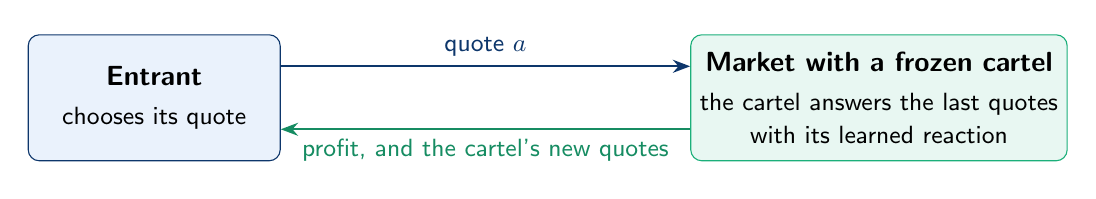
\begin{tikzpicture}[node distance=5.2cm, >={Stealth[length=2.2mm]}]
\node[draw=navy,fill=paleblue,rounded corners=4pt,minimum width=3.2cm,minimum height=1.6cm,align=center] (E) {\textbf{Entrant}\\[2pt]\small chooses its quote};
\node[draw=aqua,fill=aqua!10,rounded corners=4pt,minimum width=4.2cm,minimum height=1.6cm,align=center,right=of E] (M) {\textbf{Market with a frozen cartel}\\[2pt]\small the cartel answers the last quotes\\ \small with its learned reaction};
\draw[->,navy,thick] ([yshift=4mm]E.east) -- node[above]{\small quote $a$} ([yshift=4mm]M.west);
\draw[->,aqua!80!black,thick] ([yshift=-4mm]M.west) -- node[below]{\small profit, and the cartel's new quotes} ([yshift=-4mm]E.east);
\end{tikzpicture}
\vspace{6pt}
\begin{itemize}\small\setlength{\itemsep}{3pt}
\item Should the entrant always take the quote that earns most today?
\item What does it need to know, and can it learn that from public information?
\item What changes when the cartel keeps learning?
\item And for the least-informed participant: what is optimal, and who pays?
\end{itemize}
\takeaway{Three questions about the attacker, one per part of the lecture, and one about the ordinary trader.}
\note{Same picture as slide 2 of Lecture 15, with the ship replaced by the entrant and the insurance quote by the cartel's quote.}
\end{frame}

\begin{frame}{Against a frozen cartel, the entrant faces an MDP}
\partlabel{Lecture 15: finite MDP; the opponent as part of P}
\small
\begin{columns}[T]
\begin{column}{0.56\textwidth}
\begin{itemize}\setlength{\itemsep}{4pt}
\item \textbf{State} $x$: last period's quotes $(h_1,h_2,h_e)$, $24^3$ states.
\item \textbf{Action} $a$: the entrant's half-spread, $1,\dots,24$.
\item \textbf{Transitions} $P$: the cartel answers $x$ with its reaction $g(x)$; next state $(g(x),a)$. Deterministic.
\item \textbf{Reward} $r(x,a)$: expected profit this period, closed form.
\item \textbf{Turn limit}: 100 periods per episode.
\end{itemize}
\end{column}
\begin{column}{0.44\textwidth}
\textbf{Why this state is valid.} Each learner chooses from its own last quote and the best rival quote. Last period's quotes predict the cartel's answer and the profit.\\[6pt]
\textbf{Why the cartel is part of $P$.} Frozen, it does not respond to the entrant's \emph{policy}, only to its last quote, like the missiles of the lecture's example.
\end{column}
\end{columns}
\takeaway{The exact best response of Workshop 1 is backward induction on this MDP: value iteration with k = periods left.}
\note{Lecture 15 slides 7, 9, 12. The state must make the rest of the history irrelevant; here it does, because the learners' own state is the last quotes.}
\end{frame}

\begin{frame}{A quote that earns more today gives a policy that earns less}
\partlabel{Lecture 15 slide 15, on one of our cartels}
\small
\begin{columns}[T]
\begin{column}{0.5\textwidth}\centering
\textbf{Myopic: best profit today}\\[3pt]
\begin{tabular}{cccc}
\toprule
period & cartel & entrant & profit \\
\midrule
0 & 15, 17 & 13 & 1.21 \\
1 & 16, 13 & 12 & 1.21 \\
2 & 18, \textcolor{red}{9} & 8 & \textcolor{red}{1.05} \\
3 & \textcolor{red}{7}, 11 & 6 & \textcolor{red}{0.86} \\
\bottomrule
\end{tabular}
\end{column}
\begin{column}{0.5\textwidth}\centering
\textbf{Optimal: best total}\\[3pt]
\begin{tabular}{cccc}
\toprule
period & cartel & entrant & profit \\
\midrule
0 & 15, 17 & 12 & 1.21 \\
1 & 21, 23 & 14 & \textcolor{orange}{1.20} \\
2 & 24, 14 & 12 & 1.21 \\
3 & 14, 22 & 13 & 1.21 \\
\bottomrule
\end{tabular}
\end{column}
\end{columns}
\vspace{6pt}
Quotes in ticks; profit in rent units. In period 1 the optimal entrant gives up $0.01$ today, and the cartel stays wide.
\takeaway{The myopic entrant pushes the cartel down to 7--9 ticks. The optimal one keeps it wide and stays just inside it.}
\note{Cartel cfl\_exp2 alpha 0.1 seed 0, from python experiments/planning\_view.py. Read it like the value-iteration table of the lecture.}
\end{frame}

\begin{frame}{How much is looking ahead worth?}
\partlabel{30 two-maker cartels, ten per toxicity level}
\centering\small
\begin{tabular}{lcccc}
\toprule
policy & $\bar\alpha=0.1$ & $0.3$ & $0.5$ & simulator \\
\midrule
one-tick undercut (no model) & 0.53 & 0.48 & 0.46 & 0.50 \\
myopic (knows $P$, $\delta=0$) & 0.91 & 0.94 & 0.95 & 0.94 \\
$\delta=0.5$ & 1.20 & 1.08 & 1.16 & 1.15 \\
$\delta=0.9$ & 1.21 & 1.08 & 1.17 & 1.15 \\
optimal (100-period total) & 1.21 & 1.08 & 1.17 & 1.15 \\
\bottomrule
\end{tabular}\\[4pt]
\raggedright\footnotesize Entrant's profit per period, rent units. Columns 2--4: on the model from the starting state. Simulator: the same policies in the real simulator, toxicity levels pooled.
\takeaway{Knowing the cartel doubles the take. Looking ahead adds the rest, and a discount of 0.5 is already enough.}
\note{Lecture 15 slides 34--36: patience moves the decision. Here most of the gain comes with the first step of looking ahead.}
\end{frame}

\begin{frame}{Live: the model, period by period}
\partlabel{Demonstration}
\begin{columns}[T]
\begin{column}{0.55\textwidth}\small
\texttt{demo/index.html} replays recorded runs of the real simulator.
\begin{itemize}\setlength{\itemsep}{3pt}
\item makers' quotes against the Nash and monopoly quotes
\item each taker's order, coloured after the fact
\item running profit per maker
\end{itemize}
Controls: play, step, seek, \textbf{playback rate} 1--200 periods per second, two runs side by side.
\end{column}
\begin{column}{0.45\textwidth}\small
\textbf{Show, in this order}
\begin{enumerate}\setlength{\itemsep}{3pt}
\item The cartel alone (5 periods/s)
\item Myopic and optimal entrant side by side (step through 10 periods)
\item The public attacker: probing, then planning
\item Betting savings: never updates beside the myopic Bayesian; then a real edge, myopic beside patient (the trap)
\end{enumerate}
\end{column}
\end{columns}
\takeaway{The replay holds no model logic: a test pins it to the experiment code.}
\note{Switch to the browser. Backup if there is no browser: the GIFs in results/demo.}
\end{frame}

\begin{frame}{Without the model: build it from the public book}
\partlabel{Model-based with a learned model; 60 cartels}
\vspace{6pt}
\begin{columns}[T]
\begin{column}{0.58\textwidth}\centering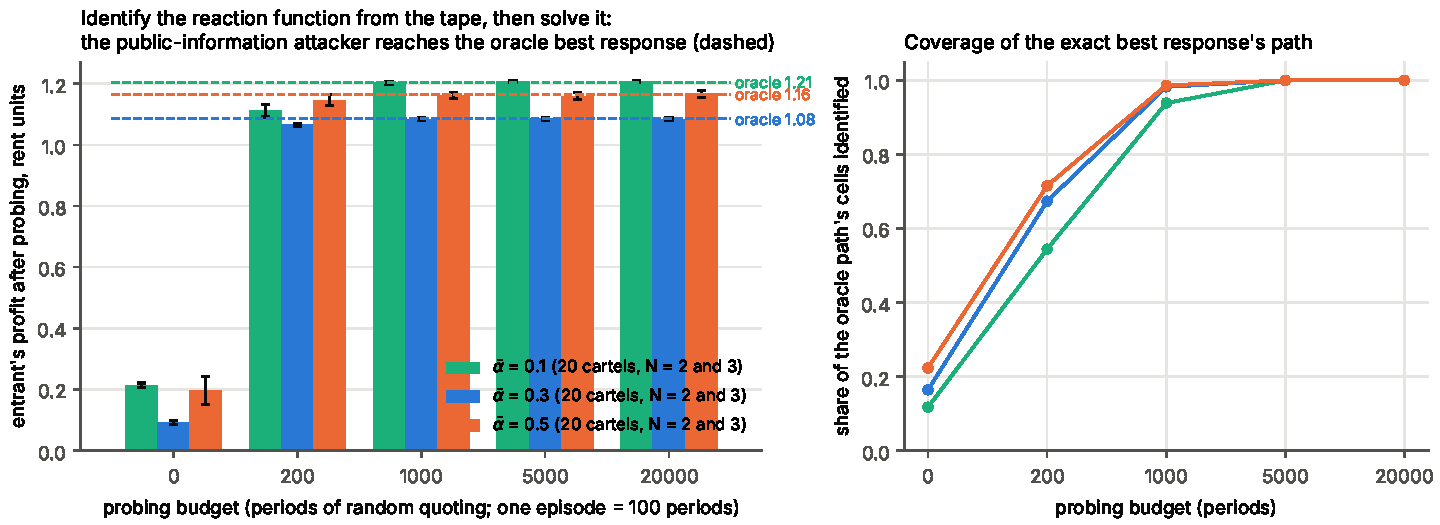
\includegraphics[width=\textwidth]{fig_public_attacker.pdf}\end{column}
\begin{column}{0.42\textwidth}\small
Every value of $P$ is on the public book: the cartel's answer appears next to the quotes it answered.\\[4pt]
Quote at random for a \textbf{probing budget}, record the answers, plan on the estimate.\\[4pt]
\stat{orange}{1000 periods}{of probing match planning with the true $P$}
\end{column}
\end{columns}
\takeaway{Probing costs profit, so the best budget is two to ten episodes. Feedback is selective: only visited states are learned.}
\note{Lecture 15: model-based planning. Next lecture is model-free; the cartel's own learners are model-free Q-learners.}
\end{frame}

\begin{frame}{When the cartel keeps learning, it is a player}
\partlabel{The game; 15 two-maker cartels, laptop size}
\centering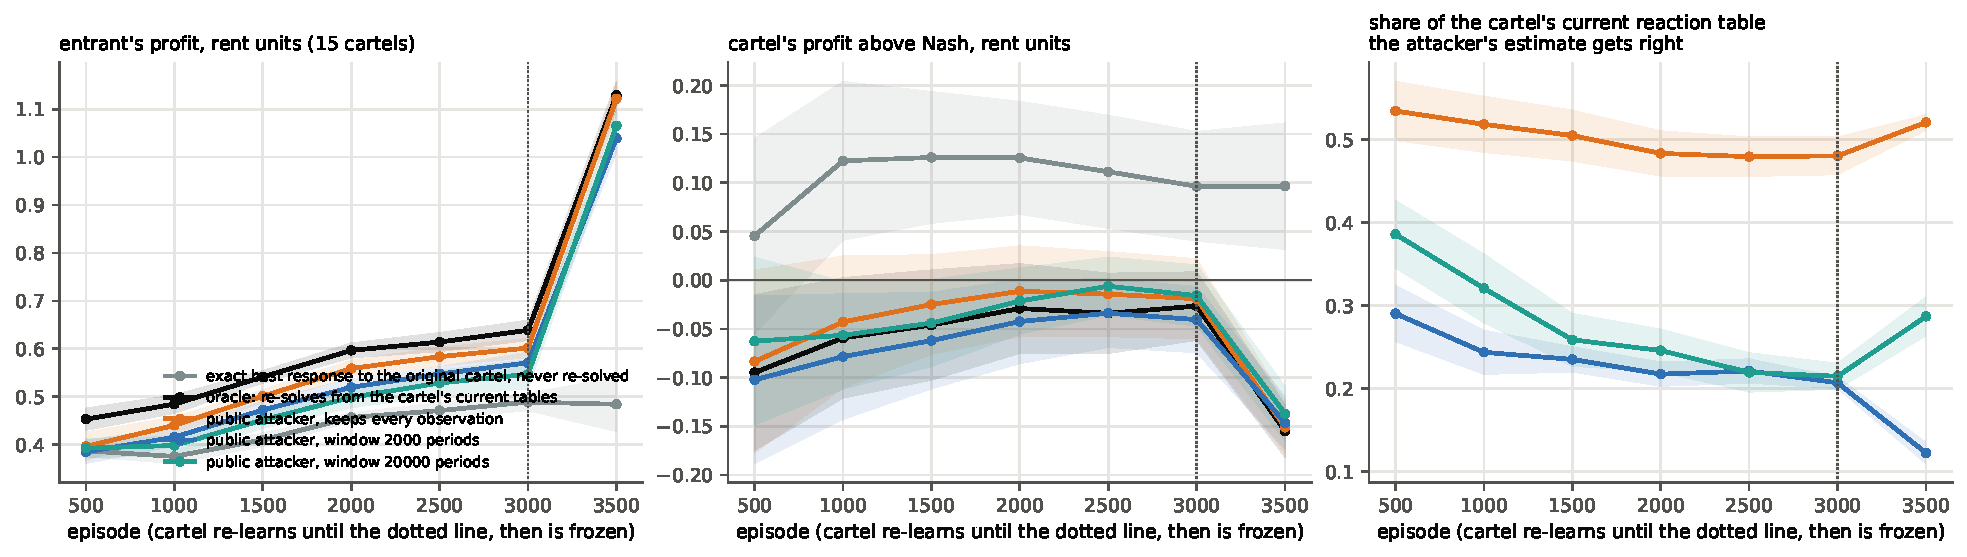
\includegraphics[width=0.9\textwidth]{fig_relearn_attack.pdf}
\takeaway{Learning lowers what the attacker can take (about 0.5 instead of 1.1), but the cartel earns about the Nash profit while it learns. We have run only the simplest version of the game.}
\note{A cartel that responds to the entrant's policy cannot be folded into P (Lecture 15 slide 9). Alternating the two sides for six rounds gave the same picture.}
\end{frame}

\begin{frame}{Identity as part of the state}
\partlabel{Data, Oct 6 -- Nov 1; RQ1}
\small
With public wallets, a maker's state can include each wallet's record, its fills and toxic fills: the lecture's belief $(n,h)$ for that wallet. On Hyperliquid, the makers who earn act on it.
\vspace{6pt}
\begin{columns}[T]
\begin{column}{0.32\textwidth}\stat{orange}{1.9--3.6$\times$}{fewer fills from previously toxic wallets for the top-10 makers}\end{column}
\begin{column}{0.32\textwidth}\stat{blue}{33 of 35}{coin-days on which the gap holds (four weeks)}\end{column}
\begin{column}{0.32\textwidth}\stat{aqua}{10 days}{for which a wallet's label stays useful}\end{column}
\end{columns}
\vspace{6pt}
\textbf{Open questions from the lecture.} Avoiding a wallet stops the feedback on it: is avoidance a trap (slide 37)? More information can lower the gains from trade in a game (slides 41--42): who bears it when wallets are public?
\takeaway{Public identity changes what the makers' state contains. Whether avoidance traps them is the next question.}
\note{Figure for questions: fig\_longwindow. Oct 29 stress episode: one identity-blind wallet absorbed the toxic flow.}
\end{frame}

\begin{frame}{The ordinary trader: who pays?}
\partlabel{The least-informed participant, same model}
\vspace{4pt}
\begin{columns}[T]
\begin{column}{0.58\textwidth}\centering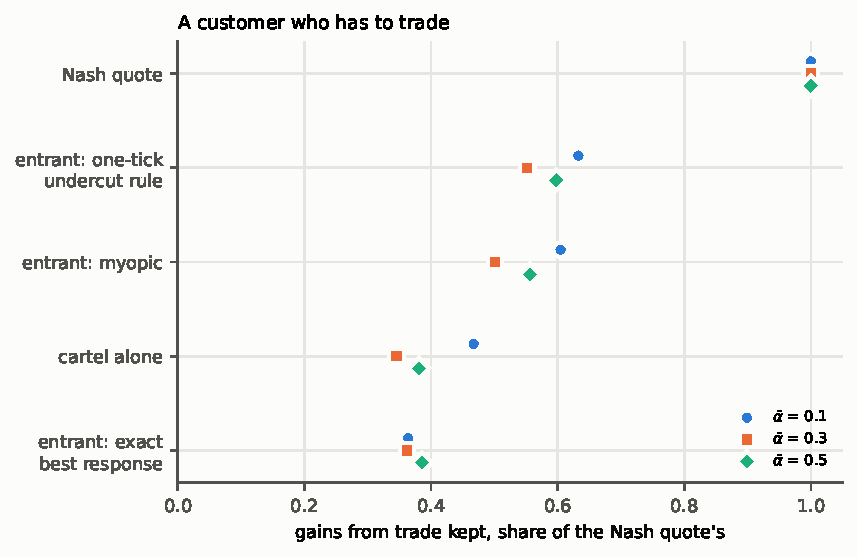
\includegraphics[width=\textwidth]{fig_retail_customer.pdf}\end{column}
\begin{column}{0.42\textwidth}\small
A customer who \textbf{has to trade} (moving savings in or out) is the model's uninformed taker. Her gains from trade fall as the quote widens.\\[5pt]
\stat{orange}{36--39\%}{of the Nash quote's gains left by the attack that is best for the attacker: no more than the cartel alone (35--47\%)}
\end{column}
\end{columns}
\takeaway{The attacker keeps the cartel wide and sits just inside it. The customer pays for both.}
\note{The myopic entrant, which pushes the cartel down, leaves her 50--60\%. 30 two-maker cartels, model paths.}
\end{frame}

\begin{frame}{Betting your savings without information: the ship again}
\partlabel{Lecture 15 part 2, with the trader as the ship}
\small
\begin{columns}[T]
\begin{column}{0.48\textwidth}
\begin{itemize}\setlength{\itemsep}{4pt}
\item A bet that is right with probability $p$ earns $(2p-1)\mu - x$: $\mu$ the mean price move, $x$ the half-spread.
\item Break-even: $p^* = \tfrac12 + x/(2\mu)$. One-tick book: $0.55$. Cartel's quotes: above 1.
\item She does not know $p$. Belief $(n,k)$: trades made, right calls. Trade = the strait (teaches), stop = the Cape (teaches nothing).
\end{itemize}
\end{column}
\begin{column}{0.52\textwidth}\centering
\footnotesize
\begin{tabular}{lccc}
\toprule
one year, optimistic prior & \multicolumn{2}{c}{no edge} & real edge \\
policy & profit & ruin & still trading \\
\midrule
never updates & $-25.0$ & 74\% & 100\% \\
myopic Bayesian & $-1.2$ & 0.3\% & 23\% \\
patient, $\delta=0.9$ & $-2.9$ & 1.0\% & 47\% \\
patient, $\delta=0.99$ & $-5.6$ & 3.8\% & 71\% \\
\bottomrule
\end{tabular}\\[3pt]
\raggedright profit in average price moves; savings 20 moves; real edge $p=0.6$.
\end{column}
\end{columns}
\takeaway{Without an edge, patience costs: information is only worth buying if an edge is plausible. With one, the myopic rule quits it 77\% of the time: the trap.}
\note{Stylised model, not investment advice. Rothschild (1974), as in the lecture.}
\end{frame}

\begin{frame}{Summary}
\partlabel{And what comes next}
\vspace{4pt}
\begin{columns}[T]
\begin{column}{0.25\textwidth}\rqbox{orange}{1~~Planning attacks}{The entrant solves an MDP. Looking ahead adds 0.13--0.30.}\end{column}
\begin{column}{0.25\textwidth}\rqbox{blue}{2~~The model is public}{The cartel's reaction is on the public book.}\end{column}
\begin{column}{0.25\textwidth}\rqbox{aqua}{3~~Learners are players}{A game. Learning did not bring the rent back.}\end{column}
\begin{column}{0.25\textwidth}\rqbox{navy}{4~~The customer pays}{The best attack leaves her no better off. Updating protects savings.}\end{column}
\end{columns}
\vspace{8pt}
\small\textbf{Next:} full-size runs; the trap question on order-level data; preprint in mid-December.\\[3pt]
\centering\texttt{github.com/pradeepu191/wargame}
\note{Close.}
\end{frame}

\begin{frame}{Backup: also explored, not claimed here}
\partlabel{Preliminary; in the repository}
\small
\begin{itemize}\setlength{\itemsep}{5pt}
\item \textbf{One-tick books (queue game).} When the spread cannot move, makers only choose to keep an order standing or not. Steering the incumbents gained nothing (3 seeds).
\item \textbf{Request allowance.} A cap on order placements removed the identity selector's edge (3 seeds).
\item \textbf{Defences on one frontier.} Maker and exchange rules against the strongest attackers; run in progress.
\end{itemize}
\vspace{4pt}
Details: \texttt{results/REPLICATION\_NOTES.md}, sections dated Nov 15--16.
\note{Only if asked.}
\end{frame}
\end{document}"
\usetheme[progressbar=frametitle,numbering=fraction,block=fill,sectionpage=none]{metropolis}
\usepackage[T1]{fontenc}
\usepackage{helvet}\renewcommand{\familydefault}{\sfdefault}
\usepackage{amsmath,amssymb}
\usepackage{booktabs}
\usepackage{tikz}
\usetikzlibrary{arrows.meta,positioning,calc,fit}
\tikzset{pl/.style={draw=#1,fill=#1!12,rounded corners=3pt,text width=3.5cm,align=left,inner sep=7pt}}
\usepackage{graphicx}
\usepackage[skins]{tcolorbox}
\ifdefined\shownotes
  \usepackage{pgfpages}
  \setbeameroption{show notes on second screen=right}
  \setbeamertemplate{note page}[plain]
  \setbeamerfont{note page}{size=\small}
\fi
\graphicspath{{../results/}{../results/live_2026_10/}}
\definecolor{ink}{HTML}{0b0b0b}
\definecolor{muted}{HTML}{52514e}
\definecolor{navy}{HTML}{0d366b}
\definecolor{blue}{HTML}{2a78d6}
\definecolor{paleblue}{HTML}{eaf2fc}
\definecolor{orange}{HTML}{eb6834}
\definecolor{paleorange}{HTML}{fdf0e9}
\definecolor{aqua}{HTML}{1baf7a}
\definecolor{red}{HTML}{e34948}
\definecolor{grey}{HTML}{9a9890}
\definecolor{paper}{HTML}{fcfcfb}
\setbeamercolor{normal text}{fg=ink,bg=paper}
\setbeamercolor{frametitle}{bg=navy,fg=white}
\setbeamercolor{progress bar}{fg=orange,bg=navy!25}
\setbeamercolor{alerted text}{fg=orange}
\setbeamercolor{block title}{bg=paleblue,fg=navy}
\setbeamercolor{block body}{bg=paleblue,fg=ink}
\setbeamercolor{itemize item}{fg=blue}
\setbeamercolor{enumerate item}{fg=blue}
\setbeamercolor{title separator}{fg=orange}
\setbeamerfont{frametitle}{size=\large,series=\bfseries}
\setbeamerfont{caption}{size=\scriptsize}
\setbeamertemplate{caption}{\insertcaption}
\setbeamertemplate{itemize items}{\textcolor{blue}{$\blacktriangleright$}}
\setlength{\leftmargini}{1.1em}
\newcommand{\Fanon}{\mathcal{F}^{\mathrm{anon}}}
\newcommand{\Fid}{\mathcal{F}^{\mathrm{id}}}
\newcommand{\For}{\mathcal{F}^{\mathrm{oracle}}}
\newcommand{\LBR}{L_{\mathrm{BR}}}
\newcommand{\takeaway}[1]{\vspace{3pt}\begin{tcolorbox}[enhanced,colback=paleorange,colframe=paleorange,borderline west={2.5pt}{0pt}{orange},boxrule=0pt,arc=1.5pt,left=6pt,right=6pt,top=3pt,bottom=3pt]\small\textbf{#1}\end{tcolorbox}}
\newcommand{\rqbox}[3]{\begin{tcolorbox}[enhanced,colback=paleblue,colframe=paleblue,borderline north={2.5pt}{0pt}{#1},boxrule=0pt,arc=1.5pt,left=6pt,right=6pt,top=5pt,bottom=5pt,height=2.6cm,valign=top]\raggedright\textcolor{#1}{\textbf{#2}}\par\vspace{3pt}\small #3\end{tcolorbox}}
\newcommand{\stat}[3]{\begin{tcolorbox}[enhanced,colback=paleblue,colframe=paleblue,borderline north={2.5pt}{0pt}{#1},boxrule=0pt,arc=1.5pt,left=5pt,right=5pt,top=4pt,bottom=4pt]\centering{\LARGE\textbf{\textcolor{#1}{#2}}}\par\vspace{2pt}{\footnotesize #3}\end{tcolorbox}}
\newcommand{\partlabel}[1]{\vspace{-10pt}\par\noindent\hfill{\scriptsize\textcolor{muted}{\textsc{#1}}}\par\vspace{-4pt}}
\newcommand{\subline}[1]{\par\vspace{3pt}{\small #1}\par}

\title{\huge Can an attacker plan against learning market makers?}
\subtitle{The entrant's problem as a Markov decision problem\\ {\small\textcolor{white!70!navy}{Rent or toxicity: strategic exploitability of learning market makers with public wallet information}}}
\author{Deepu Pradeep \quad Miguel Betran Menz}
\institute{6.S974 Games, Learning, and Security, Workshop 2 (draft)\\ Example 4: an algorithmic market with adaptive agents}
\date{November 2026}

\begin{document}
{\setbeamercolor{background canvas}{bg=navy}\setbeamercolor{normal text}{fg=white}\setbeamercolor{title}{fg=white}\setbeamercolor{subtitle}{fg=white!85!navy}\setbeamercolor{author}{fg=white}\setbeamercolor{institute}{fg=white!80!navy}\setbeamercolor{date}{fg=white!80!navy}\usebeamercolor[fg]{normal text}
\maketitle}

\begin{frame}{The words we use today}
\partlabel{Recap from Workshop 1}
\small
\begin{columns}[T]
\begin{column}{0.5\textwidth}
\begin{itemize}\setlength{\itemsep}{4pt}
\item \textbf{Maker}: posts standing offers to buy and sell. \textbf{Taker}: accepts one.
\item \textbf{Half-spread} $h$: how far a maker's prices sit from the mid, in \textbf{ticks} (smallest price step).
\item \textbf{Nash quote} $h^C$: break-even. \textbf{Monopoly quote} $h^M$: what a single maker would choose.
\end{itemize}
\end{column}
\begin{column}{0.5\textwidth}
\begin{itemize}\setlength{\itemsep}{4pt}
\item \textbf{Cartel}: learning makers that settle above Nash without communicating. \textbf{Rent}: their profit above Nash.
\item \textbf{Entrant}: the attacker, one more maker.
\item \textbf{Rent units}: profit divided by (monopoly $-$ Nash) profit. 1 is the whole rent.
\end{itemize}
\end{column}
\end{columns}
\takeaway{Workshop 1: the rent exists, and an entrant that knows how the cartel reacts takes all of it.}
\note{One slide to recall the vocabulary. The planning words come from Lecture 15 and are defined as we go.}
\end{frame}

\begin{frame}{The entrant's quote changes the cartel it faces tomorrow}
\partlabel{The frame of Lecture 15}
\centering
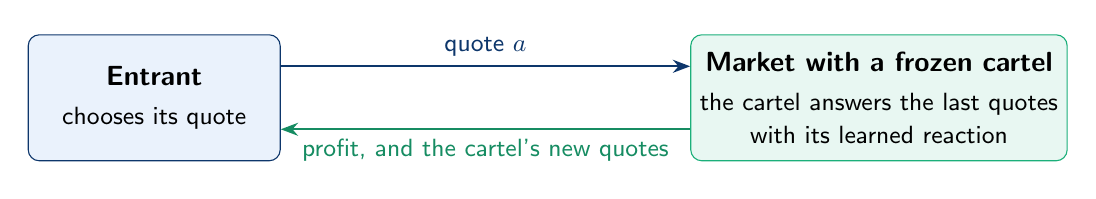
\begin{tikzpicture}[node distance=5.2cm, >={Stealth[length=2.2mm]}]
\node[draw=navy,fill=paleblue,rounded corners=4pt,minimum width=3.2cm,minimum height=1.6cm,align=center] (E) {\textbf{Entrant}\\[2pt]\small chooses its quote};
\node[draw=aqua,fill=aqua!10,rounded corners=4pt,minimum width=4.2cm,minimum height=1.6cm,align=center,right=of E] (M) {\textbf{Market with a frozen cartel}\\[2pt]\small the cartel answers the last quotes\\ \small with its learned reaction};
\draw[->,navy,thick] ([yshift=4mm]E.east) -- node[above]{\small quote $a$} ([yshift=4mm]M.west);
\draw[->,aqua!80!black,thick] ([yshift=-4mm]M.west) -- node[below]{\small profit, and the cartel's new quotes} ([yshift=-4mm]E.east);
\end{tikzpicture}
\vspace{6pt}
\begin{itemize}\small\setlength{\itemsep}{3pt}
\item Should the entrant always take the quote that earns most today?
\item What does it need to know, and can it learn that from public information?
\item What changes when the cartel keeps learning?
\item And for the least-informed participant: what is optimal, and who pays?
\end{itemize}
\takeaway{Three questions about the attacker, one per part of the lecture, and one about the ordinary trader.}
\note{Same picture as slide 2 of Lecture 15, with the ship replaced by the entrant and the insurance quote by the cartel's quote.}
\end{frame}

\begin{frame}{Against a frozen cartel, the entrant faces an MDP}
\partlabel{Lecture 15: finite MDP; the opponent as part of P}
\small
\begin{columns}[T]
\begin{column}{0.56\textwidth}
\begin{itemize}\setlength{\itemsep}{4pt}
\item \textbf{State} $x$: last period's quotes $(h_1,h_2,h_e)$, $24^3$ states.
\item \textbf{Action} $a$: the entrant's half-spread, $1,\dots,24$.
\item \textbf{Transitions} $P$: the cartel answers $x$ with its reaction $g(x)$; next state $(g(x),a)$. Deterministic.
\item \textbf{Reward} $r(x,a)$: expected profit this period, closed form.
\item \textbf{Turn limit}: 100 periods per episode.
\end{itemize}
\end{column}
\begin{column}{0.44\textwidth}
\textbf{Why this state is valid.} Each learner chooses from its own last quote and the best rival quote. Last period's quotes predict the cartel's answer and the profit.\\[6pt]
\textbf{Why the cartel is part of $P$.} Frozen, it does not respond to the entrant's \emph{policy}, only to its last quote, like the missiles of the lecture's example.
\end{column}
\end{columns}
\takeaway{The exact best response of Workshop 1 is backward induction on this MDP: value iteration with k = periods left.}
\note{Lecture 15 slides 7, 9, 12. The state must make the rest of the history irrelevant; here it does, because the learners' own state is the last quotes.}
\end{frame}

\begin{frame}{A quote that earns more today gives a policy that earns less}
\partlabel{Lecture 15 slide 15, on one of our cartels}
\small
\begin{columns}[T]
\begin{column}{0.5\textwidth}\centering
\textbf{Myopic: best profit today}\\[3pt]
\begin{tabular}{cccc}
\toprule
period & cartel & entrant & profit \\
\midrule
0 & 15, 17 & 13 & 1.21 \\
1 & 16, 13 & 12 & 1.21 \\
2 & 18, \textcolor{red}{9} & 8 & \textcolor{red}{1.05} \\
3 & \textcolor{red}{7}, 11 & 6 & \textcolor{red}{0.86} \\
\bottomrule
\end{tabular}
\end{column}
\begin{column}{0.5\textwidth}\centering
\textbf{Optimal: best total}\\[3pt]
\begin{tabular}{cccc}
\toprule
period & cartel & entrant & profit \\
\midrule
0 & 15, 17 & 12 & 1.21 \\
1 & 21, 23 & 14 & \textcolor{orange}{1.20} \\
2 & 24, 14 & 12 & 1.21 \\
3 & 14, 22 & 13 & 1.21 \\
\bottomrule
\end{tabular}
\end{column}
\end{columns}
\vspace{6pt}
Quotes in ticks; profit in rent units. In period 1 the optimal entrant gives up $0.01$ today, and the cartel stays wide.
\takeaway{The myopic entrant pushes the cartel down to 7--9 ticks. The optimal one keeps it wide and stays just inside it.}
\note{Cartel cfl\_exp2 alpha 0.1 seed 0, from python experiments/planning\_view.py. Read it like the value-iteration table of the lecture.}
\end{frame}

\begin{frame}{How much is looking ahead worth?}
\partlabel{30 two-maker cartels, ten per toxicity level}
\centering\small
\begin{tabular}{lcccc}
\toprule
policy & $\bar\alpha=0.1$ & $0.3$ & $0.5$ & simulator \\
\midrule
one-tick undercut (no model) & 0.53 & 0.48 & 0.46 & 0.50 \\
myopic (knows $P$, $\delta=0$) & 0.91 & 0.94 & 0.95 & 0.94 \\
$\delta=0.5$ & 1.20 & 1.08 & 1.16 & 1.15 \\
$\delta=0.9$ & 1.21 & 1.08 & 1.17 & 1.15 \\
optimal (100-period total) & 1.21 & 1.08 & 1.17 & 1.15 \\
\bottomrule
\end{tabular}\\[4pt]
\raggedright\footnotesize Entrant's profit per period, rent units. Columns 2--4: on the model from the starting state. Simulator: the same policies in the real simulator, toxicity levels pooled.
\takeaway{Knowing the cartel doubles the take. Looking ahead adds the rest, and a discount of 0.5 is already enough.}
\note{Lecture 15 slides 34--36: patience moves the decision. Here most of the gain comes with the first step of looking ahead.}
\end{frame}

\begin{frame}{Live: the model, period by period}
\partlabel{Demonstration}
\begin{columns}[T]
\begin{column}{0.55\textwidth}\small
\texttt{demo/index.html} replays recorded runs of the real simulator.
\begin{itemize}\setlength{\itemsep}{3pt}
\item makers' quotes against the Nash and monopoly quotes
\item each taker's order, coloured after the fact
\item running profit per maker
\end{itemize}
Controls: play, step, seek, \textbf{playback rate} 1--200 periods per second, two runs side by side.
\end{column}
\begin{column}{0.45\textwidth}\small
\textbf{Show, in this order}
\begin{enumerate}\setlength{\itemsep}{3pt}
\item The cartel alone (5 periods/s)
\item Myopic and optimal entrant side by side (step through 10 periods)
\item The public attacker: probing, then planning
\item Betting savings: never updates beside the myopic Bayesian; then a real edge, myopic beside patient (the trap)
\end{enumerate}
\end{column}
\end{columns}
\takeaway{The replay holds no model logic: a test pins it to the experiment code.}
\note{Switch to the browser. Backup if there is no browser: the GIFs in results/demo.}
\end{frame}

\begin{frame}{Without the model: build it from the public book}
\partlabel{Model-based with a learned model; 60 cartels}
\vspace{6pt}
\begin{columns}[T]
\begin{column}{0.58\textwidth}\centering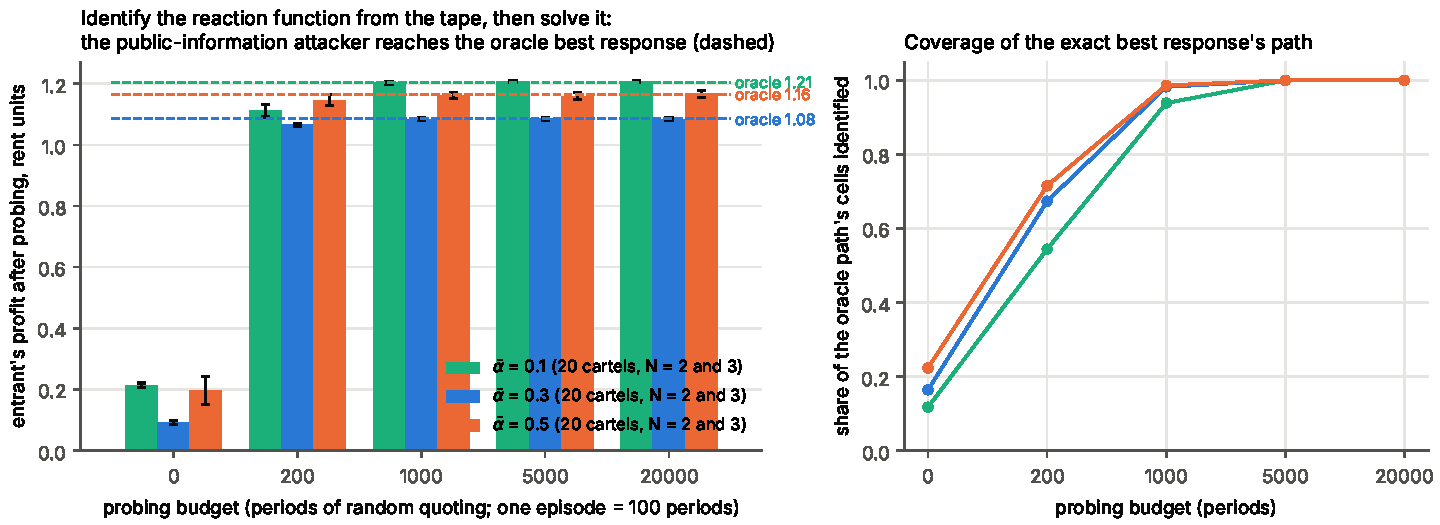
\includegraphics[width=\textwidth]{fig_public_attacker.pdf}\end{column}
\begin{column}{0.42\textwidth}\small
Every value of $P$ is on the public book: the cartel's answer appears next to the quotes it answered.\\[4pt]
Quote at random for a \textbf{probing budget}, record the answers, plan on the estimate.\\[4pt]
\stat{orange}{1000 periods}{of probing match planning with the true $P$}
\end{column}
\end{columns}
\takeaway{Probing costs profit, so the best budget is two to ten episodes. Feedback is selective: only visited states are learned.}
\note{Lecture 15: model-based planning. Next lecture is model-free; the cartel's own learners are model-free Q-learners.}
\end{frame}

\begin{frame}{When the cartel keeps learning, it is a player}
\partlabel{The game; 15 two-maker cartels, laptop size}
\centering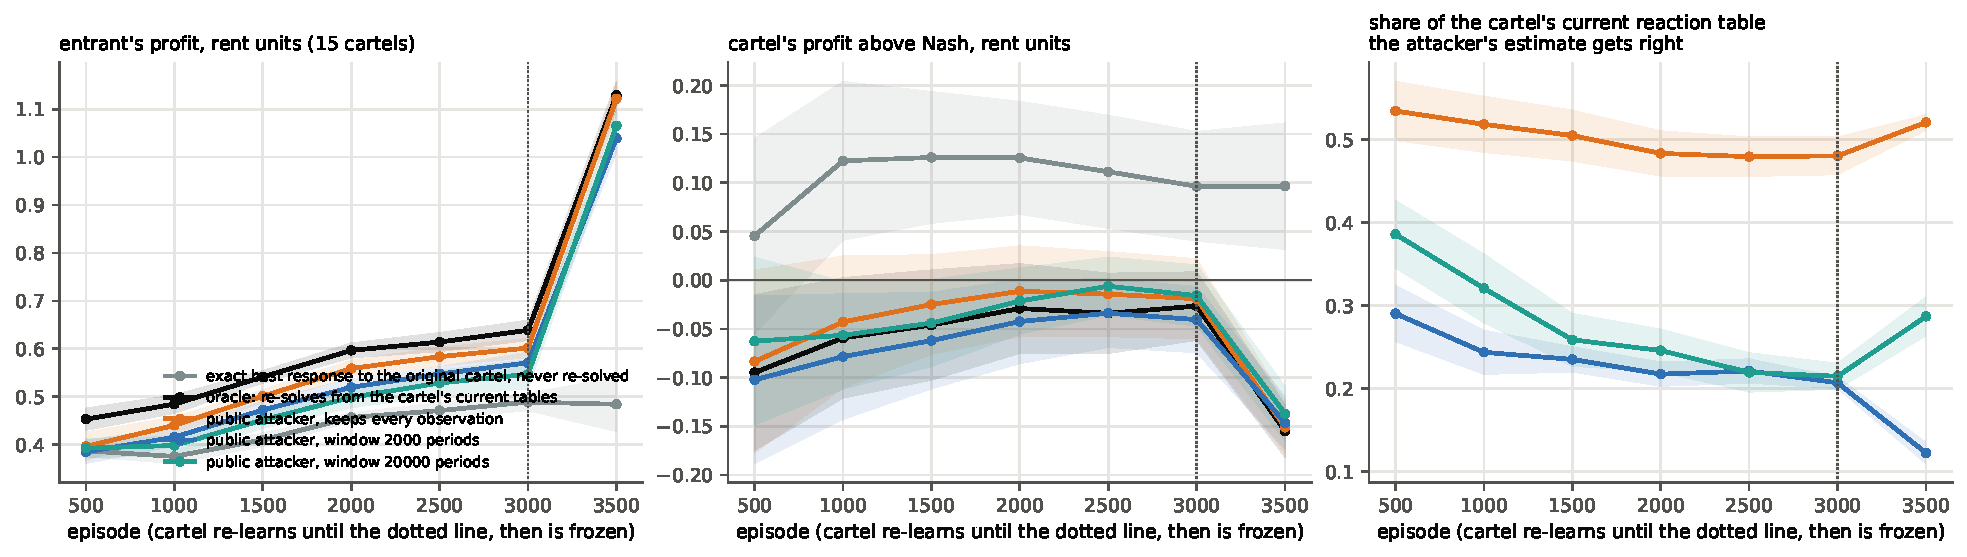
\includegraphics[width=0.9\textwidth]{fig_relearn_attack.pdf}
\takeaway{Learning lowers what the attacker can take (about 0.5 instead of 1.1), but the cartel earns about the Nash profit while it learns. We have run only the simplest version of the game.}
\note{A cartel that responds to the entrant's policy cannot be folded into P (Lecture 15 slide 9). Alternating the two sides for six rounds gave the same picture.}
\end{frame}

\begin{frame}{Identity as part of the state}
\partlabel{Data, Oct 6 -- Nov 1; RQ1}
\small
With public wallets, a maker's state can include each wallet's record, its fills and toxic fills: the lecture's belief $(n,h)$ for that wallet. On Hyperliquid, the makers who earn act on it.
\vspace{6pt}
\begin{columns}[T]
\begin{column}{0.32\textwidth}\stat{orange}{1.9--3.6$\times$}{fewer fills from previously toxic wallets for the top-10 makers}\end{column}
\begin{column}{0.32\textwidth}\stat{blue}{33 of 35}{coin-days on which the gap holds (four weeks)}\end{column}
\begin{column}{0.32\textwidth}\stat{aqua}{10 days}{for which a wallet's label stays useful}\end{column}
\end{columns}
\vspace{6pt}
\textbf{Open questions from the lecture.} Avoiding a wallet stops the feedback on it: is avoidance a trap (slide 37)? More information can lower the gains from trade in a game (slides 41--42): who bears it when wallets are public?
\takeaway{Public identity changes what the makers' state contains. Whether avoidance traps them is the next question.}
\note{Figure for questions: fig\_longwindow. Oct 29 stress episode: one identity-blind wallet absorbed the toxic flow.}
\end{frame}

\begin{frame}{The ordinary trader: who pays?}
\partlabel{The least-informed participant, same model}
\vspace{4pt}
\begin{columns}[T]
\begin{column}{0.58\textwidth}\centering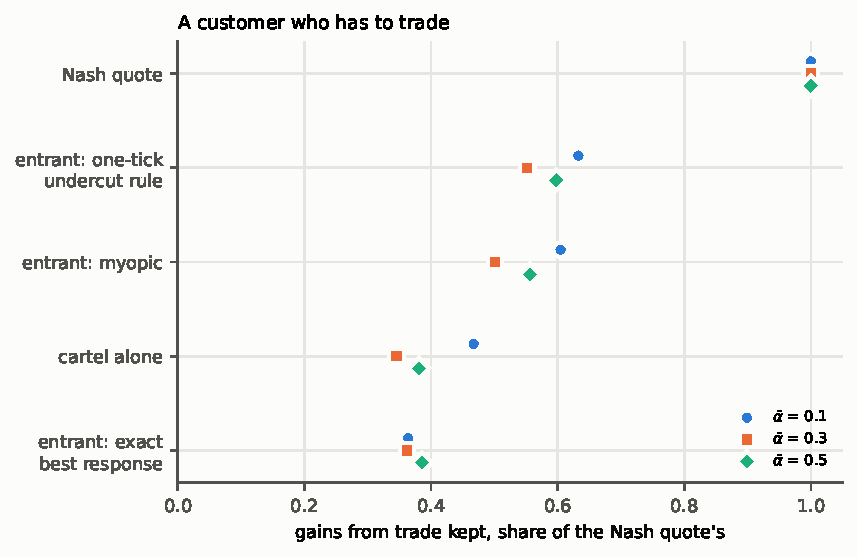
\includegraphics[width=\textwidth]{fig_retail_customer.pdf}\end{column}
\begin{column}{0.42\textwidth}\small
A customer who \textbf{has to trade} (moving savings in or out) is the model's uninformed taker. Her gains from trade fall as the quote widens.\\[5pt]
\stat{orange}{36--39\%}{of the Nash quote's gains left by the attack that is best for the attacker: no more than the cartel alone (35--47\%)}
\end{column}
\end{columns}
\takeaway{The attacker keeps the cartel wide and sits just inside it. The customer pays for both.}
\note{The myopic entrant, which pushes the cartel down, leaves her 50--60\%. 30 two-maker cartels, model paths.}
\end{frame}

\begin{frame}{Betting your savings without information: the ship again}
\partlabel{Lecture 15 part 2, with the trader as the ship}
\small
\begin{columns}[T]
\begin{column}{0.48\textwidth}
\begin{itemize}\setlength{\itemsep}{4pt}
\item A bet that is right with probability $p$ earns $(2p-1)\mu - x$: $\mu$ the mean price move, $x$ the half-spread.
\item Break-even: $p^* = \tfrac12 + x/(2\mu)$. One-tick book: $0.55$. Cartel's quotes: above 1.
\item She does not know $p$. Belief $(n,k)$: trades made, right calls. Trade = the strait (teaches), stop = the Cape (teaches nothing).
\end{itemize}
\end{column}
\begin{column}{0.52\textwidth}\centering
\footnotesize
\begin{tabular}{lccc}
\toprule
one year, optimistic prior & \multicolumn{2}{c}{no edge} & real edge \\
policy & profit & ruin & still trading \\
\midrule
never updates & $-25.0$ & 74\% & 100\% \\
myopic Bayesian & $-1.2$ & 0.3\% & 23\% \\
patient, $\delta=0.9$ & $-2.9$ & 1.0\% & 47\% \\
patient, $\delta=0.99$ & $-5.6$ & 3.8\% & 71\% \\
\bottomrule
\end{tabular}\\[3pt]
\raggedright profit in average price moves; savings 20 moves; real edge $p=0.6$.
\end{column}
\end{columns}
\takeaway{Without an edge, patience costs: information is only worth buying if an edge is plausible. With one, the myopic rule quits it 77\% of the time: the trap.}
\note{Stylised model, not investment advice. Rothschild (1974), as in the lecture.}
\end{frame}

\begin{frame}{Summary}
\partlabel{And what comes next}
\vspace{4pt}
\begin{columns}[T]
\begin{column}{0.25\textwidth}\rqbox{orange}{1~~Planning attacks}{The entrant solves an MDP. Looking ahead adds 0.13--0.30.}\end{column}
\begin{column}{0.25\textwidth}\rqbox{blue}{2~~The model is public}{The cartel's reaction is on the public book.}\end{column}
\begin{column}{0.25\textwidth}\rqbox{aqua}{3~~Learners are players}{A game. Learning did not bring the rent back.}\end{column}
\begin{column}{0.25\textwidth}\rqbox{navy}{4~~The customer pays}{The best attack leaves her no better off. Updating protects savings.}\end{column}
\end{columns}
\vspace{8pt}
\small\textbf{Next:} full-size runs; the trap question on order-level data; preprint in mid-December.\\[3pt]
\centering\texttt{github.com/pradeepu191/wargame}
\note{Close.}
\end{frame}

\begin{frame}{Backup: also explored, not claimed here}
\partlabel{Preliminary; in the repository}
\small
\begin{itemize}\setlength{\itemsep}{5pt}
\item \textbf{One-tick books (queue game).} When the spread cannot move, makers only choose to keep an order standing or not. Steering the incumbents gained nothing (3 seeds).
\item \textbf{Request allowance.} A cap on order placements removed the identity selector's edge (3 seeds).
\item \textbf{Defences on one frontier.} Maker and exchange rules against the strongest attackers; run in progress.
\end{itemize}
\vspace{4pt}
Details: \texttt{results/REPLICATION\_NOTES.md}, sections dated Nov 15--16.
\note{Only if asked.}
\end{frame}
\end{document}"
\usetheme[progressbar=frametitle,numbering=fraction,block=fill,sectionpage=none]{metropolis}
\usepackage[T1]{fontenc}
\usepackage{helvet}\renewcommand{\familydefault}{\sfdefault}
\usepackage{amsmath,amssymb}
\usepackage{booktabs}
\usepackage{tikz}
\usetikzlibrary{arrows.meta,positioning,calc,fit}
\tikzset{pl/.style={draw=#1,fill=#1!12,rounded corners=3pt,text width=3.5cm,align=left,inner sep=7pt}}
\usepackage{graphicx}
\usepackage[skins]{tcolorbox}
\ifdefined\shownotes
  \usepackage{pgfpages}
  \setbeameroption{show notes on second screen=right}
  \setbeamertemplate{note page}[plain]
  \setbeamerfont{note page}{size=\small}
\fi
\graphicspath{{../results/}{../results/live_2026_10/}}
\definecolor{ink}{HTML}{0b0b0b}
\definecolor{muted}{HTML}{52514e}
\definecolor{navy}{HTML}{0d366b}
\definecolor{blue}{HTML}{2a78d6}
\definecolor{paleblue}{HTML}{eaf2fc}
\definecolor{orange}{HTML}{eb6834}
\definecolor{paleorange}{HTML}{fdf0e9}
\definecolor{aqua}{HTML}{1baf7a}
\definecolor{red}{HTML}{e34948}
\definecolor{grey}{HTML}{9a9890}
\definecolor{paper}{HTML}{fcfcfb}
\setbeamercolor{normal text}{fg=ink,bg=paper}
\setbeamercolor{frametitle}{bg=navy,fg=white}
\setbeamercolor{progress bar}{fg=orange,bg=navy!25}
\setbeamercolor{alerted text}{fg=orange}
\setbeamercolor{block title}{bg=paleblue,fg=navy}
\setbeamercolor{block body}{bg=paleblue,fg=ink}
\setbeamercolor{itemize item}{fg=blue}
\setbeamercolor{enumerate item}{fg=blue}
\setbeamercolor{title separator}{fg=orange}
\setbeamerfont{frametitle}{size=\large,series=\bfseries}
\setbeamerfont{caption}{size=\scriptsize}
\setbeamertemplate{caption}{\insertcaption}
\setbeamertemplate{itemize items}{\textcolor{blue}{$\blacktriangleright$}}
\setlength{\leftmargini}{1.1em}
\newcommand{\Fanon}{\mathcal{F}^{\mathrm{anon}}}
\newcommand{\Fid}{\mathcal{F}^{\mathrm{id}}}
\newcommand{\For}{\mathcal{F}^{\mathrm{oracle}}}
\newcommand{\LBR}{L_{\mathrm{BR}}}
\newcommand{\takeaway}[1]{\vspace{3pt}\begin{tcolorbox}[enhanced,colback=paleorange,colframe=paleorange,borderline west={2.5pt}{0pt}{orange},boxrule=0pt,arc=1.5pt,left=6pt,right=6pt,top=3pt,bottom=3pt]\small\textbf{#1}\end{tcolorbox}}
\newcommand{\rqbox}[3]{\begin{tcolorbox}[enhanced,colback=paleblue,colframe=paleblue,borderline north={2.5pt}{0pt}{#1},boxrule=0pt,arc=1.5pt,left=6pt,right=6pt,top=5pt,bottom=5pt,height=2.6cm,valign=top]\raggedright\textcolor{#1}{\textbf{#2}}\par\vspace{3pt}\small #3\end{tcolorbox}}
\newcommand{\stat}[3]{\begin{tcolorbox}[enhanced,colback=paleblue,colframe=paleblue,borderline north={2.5pt}{0pt}{#1},boxrule=0pt,arc=1.5pt,left=5pt,right=5pt,top=4pt,bottom=4pt]\centering{\LARGE\textbf{\textcolor{#1}{#2}}}\par\vspace{2pt}{\footnotesize #3}\end{tcolorbox}}
\newcommand{\partlabel}[1]{\vspace{-10pt}\par\noindent\hfill{\scriptsize\textcolor{muted}{\textsc{#1}}}\par\vspace{-4pt}}
\newcommand{\subline}[1]{\par\vspace{3pt}{\small #1}\par}

\title{\huge Can an attacker plan against learning market makers?}
\subtitle{The entrant's problem as a Markov decision problem\\ {\small\textcolor{white!70!navy}{Rent or toxicity: strategic exploitability of learning market makers with public wallet information}}}
\author{Deepu Pradeep \quad Miguel Betran Menz}
\institute{6.S974 Games, Learning, and Security, Workshop 2 (draft)\\ Example 4: an algorithmic market with adaptive agents}
\date{November 2026}

\begin{document}
{\setbeamercolor{background canvas}{bg=navy}\setbeamercolor{normal text}{fg=white}\setbeamercolor{title}{fg=white}\setbeamercolor{subtitle}{fg=white!85!navy}\setbeamercolor{author}{fg=white}\setbeamercolor{institute}{fg=white!80!navy}\setbeamercolor{date}{fg=white!80!navy}\usebeamercolor[fg]{normal text}
\maketitle}

\begin{frame}{The words we use today}
\partlabel{Recap from Workshop 1}
\small
\begin{columns}[T]
\begin{column}{0.5\textwidth}
\begin{itemize}\setlength{\itemsep}{4pt}
\item \textbf{Maker}: posts standing offers to buy and sell. \textbf{Taker}: accepts one.
\item \textbf{Half-spread} $h$: how far a maker's prices sit from the mid, in \textbf{ticks} (smallest price step).
\item \textbf{Nash quote} $h^C$: break-even. \textbf{Monopoly quote} $h^M$: what a single maker would choose.
\end{itemize}
\end{column}
\begin{column}{0.5\textwidth}
\begin{itemize}\setlength{\itemsep}{4pt}
\item \textbf{Cartel}: learning makers that settle above Nash without communicating. \textbf{Rent}: their profit above Nash.
\item \textbf{Entrant}: the attacker, one more maker.
\item \textbf{Rent units}: profit divided by (monopoly $-$ Nash) profit. 1 is the whole rent.
\end{itemize}
\end{column}
\end{columns}
\takeaway{Workshop 1: the rent exists, and an entrant that knows how the cartel reacts takes all of it.}
\note{One slide to recall the vocabulary. The planning words come from Lecture 15 and are defined as we go.}
\end{frame}

\begin{frame}{The entrant's quote changes the cartel it faces tomorrow}
\partlabel{The frame of Lecture 15}
\centering
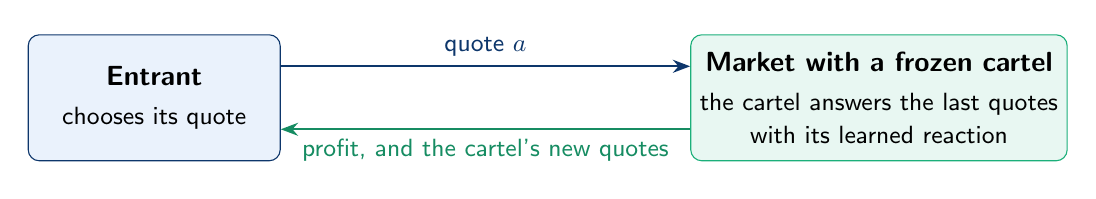
\begin{tikzpicture}[node distance=5.2cm, >={Stealth[length=2.2mm]}]
\node[draw=navy,fill=paleblue,rounded corners=4pt,minimum width=3.2cm,minimum height=1.6cm,align=center] (E) {\textbf{Entrant}\\[2pt]\small chooses its quote};
\node[draw=aqua,fill=aqua!10,rounded corners=4pt,minimum width=4.2cm,minimum height=1.6cm,align=center,right=of E] (M) {\textbf{Market with a frozen cartel}\\[2pt]\small the cartel answers the last quotes\\ \small with its learned reaction};
\draw[->,navy,thick] ([yshift=4mm]E.east) -- node[above]{\small quote $a$} ([yshift=4mm]M.west);
\draw[->,aqua!80!black,thick] ([yshift=-4mm]M.west) -- node[below]{\small profit, and the cartel's new quotes} ([yshift=-4mm]E.east);
\end{tikzpicture}
\vspace{6pt}
\begin{itemize}\small\setlength{\itemsep}{3pt}
\item Should the entrant always take the quote that earns most today?
\item What does it need to know, and can it learn that from public information?
\item What changes when the cartel keeps learning?
\item And for the least-informed participant: what is optimal, and who pays?
\end{itemize}
\takeaway{Three questions about the attacker, one per part of the lecture, and one about the ordinary trader.}
\note{Same picture as slide 2 of Lecture 15, with the ship replaced by the entrant and the insurance quote by the cartel's quote.}
\end{frame}

\begin{frame}{Against a frozen cartel, the entrant faces an MDP}
\partlabel{Lecture 15: finite MDP; the opponent as part of P}
\small
\begin{columns}[T]
\begin{column}{0.56\textwidth}
\begin{itemize}\setlength{\itemsep}{4pt}
\item \textbf{State} $x$: last period's quotes $(h_1,h_2,h_e)$, $24^3$ states.
\item \textbf{Action} $a$: the entrant's half-spread, $1,\dots,24$.
\item \textbf{Transitions} $P$: the cartel answers $x$ with its reaction $g(x)$; next state $(g(x),a)$. Deterministic.
\item \textbf{Reward} $r(x,a)$: expected profit this period, closed form.
\item \textbf{Turn limit}: 100 periods per episode.
\end{itemize}
\end{column}
\begin{column}{0.44\textwidth}
\textbf{Why this state is valid.} Each learner chooses from its own last quote and the best rival quote. Last period's quotes predict the cartel's answer and the profit.\\[6pt]
\textbf{Why the cartel is part of $P$.} Frozen, it does not respond to the entrant's \emph{policy}, only to its last quote, like the missiles of the lecture's example.
\end{column}
\end{columns}
\takeaway{The exact best response of Workshop 1 is backward induction on this MDP: value iteration with k = periods left.}
\note{Lecture 15 slides 7, 9, 12. The state must make the rest of the history irrelevant; here it does, because the learners' own state is the last quotes.}
\end{frame}

\begin{frame}{A quote that earns more today gives a policy that earns less}
\partlabel{Lecture 15 slide 15, on one of our cartels}
\small
\begin{columns}[T]
\begin{column}{0.5\textwidth}\centering
\textbf{Myopic: best profit today}\\[3pt]
\begin{tabular}{cccc}
\toprule
period & cartel & entrant & profit \\
\midrule
0 & 15, 17 & 13 & 1.21 \\
1 & 16, 13 & 12 & 1.21 \\
2 & 18, \textcolor{red}{9} & 8 & \textcolor{red}{1.05} \\
3 & \textcolor{red}{7}, 11 & 6 & \textcolor{red}{0.86} \\
\bottomrule
\end{tabular}
\end{column}
\begin{column}{0.5\textwidth}\centering
\textbf{Optimal: best total}\\[3pt]
\begin{tabular}{cccc}
\toprule
period & cartel & entrant & profit \\
\midrule
0 & 15, 17 & 12 & 1.21 \\
1 & 21, 23 & 14 & \textcolor{orange}{1.20} \\
2 & 24, 14 & 12 & 1.21 \\
3 & 14, 22 & 13 & 1.21 \\
\bottomrule
\end{tabular}
\end{column}
\end{columns}
\vspace{6pt}
Quotes in ticks; profit in rent units. In period 1 the optimal entrant gives up $0.01$ today, and the cartel stays wide.
\takeaway{The myopic entrant pushes the cartel down to 7--9 ticks. The optimal one keeps it wide and stays just inside it.}
\note{Cartel cfl\_exp2 alpha 0.1 seed 0, from python experiments/planning\_view.py. Read it like the value-iteration table of the lecture.}
\end{frame}

\begin{frame}{How much is looking ahead worth?}
\partlabel{30 two-maker cartels, ten per toxicity level}
\centering\small
\begin{tabular}{lcccc}
\toprule
policy & $\bar\alpha=0.1$ & $0.3$ & $0.5$ & simulator \\
\midrule
one-tick undercut (no model) & 0.53 & 0.48 & 0.46 & 0.50 \\
myopic (knows $P$, $\delta=0$) & 0.91 & 0.94 & 0.95 & 0.94 \\
$\delta=0.5$ & 1.20 & 1.08 & 1.16 & 1.15 \\
$\delta=0.9$ & 1.21 & 1.08 & 1.17 & 1.15 \\
optimal (100-period total) & 1.21 & 1.08 & 1.17 & 1.15 \\
\bottomrule
\end{tabular}\\[4pt]
\raggedright\footnotesize Entrant's profit per period, rent units. Columns 2--4: on the model from the starting state. Simulator: the same policies in the real simulator, toxicity levels pooled.
\takeaway{Knowing the cartel doubles the take. Looking ahead adds the rest, and a discount of 0.5 is already enough.}
\note{Lecture 15 slides 34--36: patience moves the decision. Here most of the gain comes with the first step of looking ahead.}
\end{frame}

\begin{frame}{Live: the model, period by period}
\partlabel{Demonstration}
\begin{columns}[T]
\begin{column}{0.55\textwidth}\small
\texttt{demo/index.html} replays recorded runs of the real simulator.
\begin{itemize}\setlength{\itemsep}{3pt}
\item makers' quotes against the Nash and monopoly quotes
\item each taker's order, coloured after the fact
\item running profit per maker
\end{itemize}
Controls: play, step, seek, \textbf{playback rate} 1--200 periods per second, two runs side by side.
\end{column}
\begin{column}{0.45\textwidth}\small
\textbf{Show, in this order}
\begin{enumerate}\setlength{\itemsep}{3pt}
\item The cartel alone (5 periods/s)
\item Myopic and optimal entrant side by side (step through 10 periods)
\item The public attacker: probing, then planning
\item Betting savings: never updates beside the myopic Bayesian; then a real edge, myopic beside patient (the trap)
\end{enumerate}
\end{column}
\end{columns}
\takeaway{The replay holds no model logic: a test pins it to the experiment code.}
\note{Switch to the browser. Backup if there is no browser: the GIFs in results/demo.}
\end{frame}

\begin{frame}{Without the model: build it from the public book}
\partlabel{Model-based with a learned model; 60 cartels}
\vspace{6pt}
\begin{columns}[T]
\begin{column}{0.58\textwidth}\centering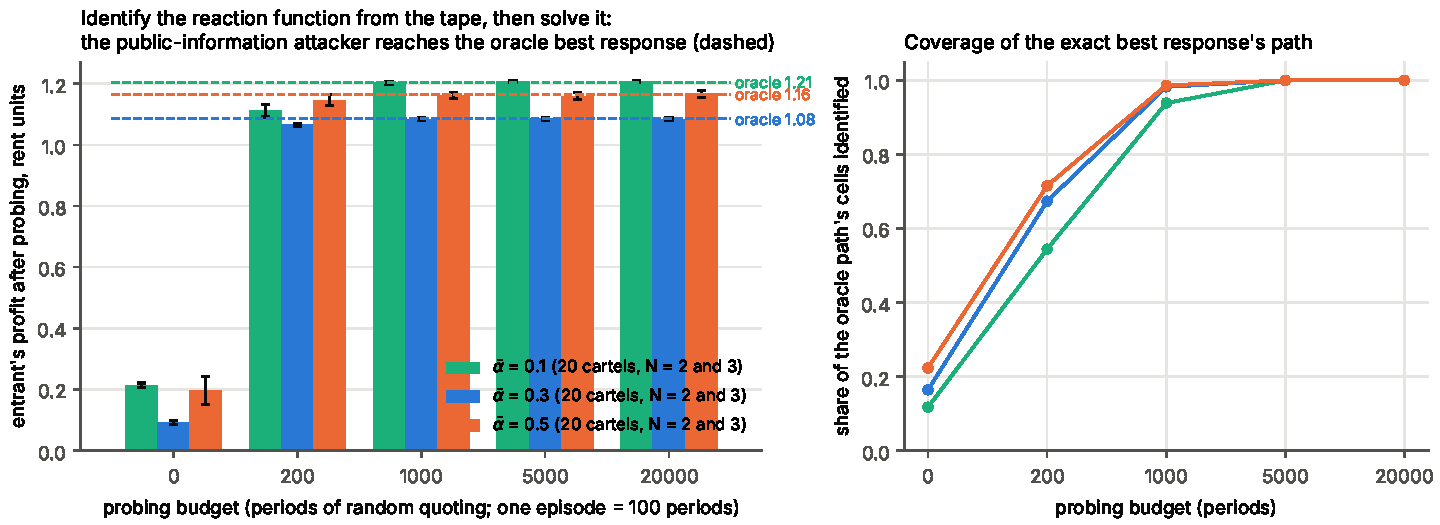
\includegraphics[width=\textwidth]{fig_public_attacker.pdf}\end{column}
\begin{column}{0.42\textwidth}\small
Every value of $P$ is on the public book: the cartel's answer appears next to the quotes it answered.\\[4pt]
Quote at random for a \textbf{probing budget}, record the answers, plan on the estimate.\\[4pt]
\stat{orange}{1000 periods}{of probing match planning with the true $P$}
\end{column}
\end{columns}
\takeaway{Probing costs profit, so the best budget is two to ten episodes. Feedback is selective: only visited states are learned.}
\note{Lecture 15: model-based planning. Next lecture is model-free; the cartel's own learners are model-free Q-learners.}
\end{frame}

\begin{frame}{When the cartel keeps learning, it is a player}
\partlabel{The game; 15 two-maker cartels, laptop size}
\centering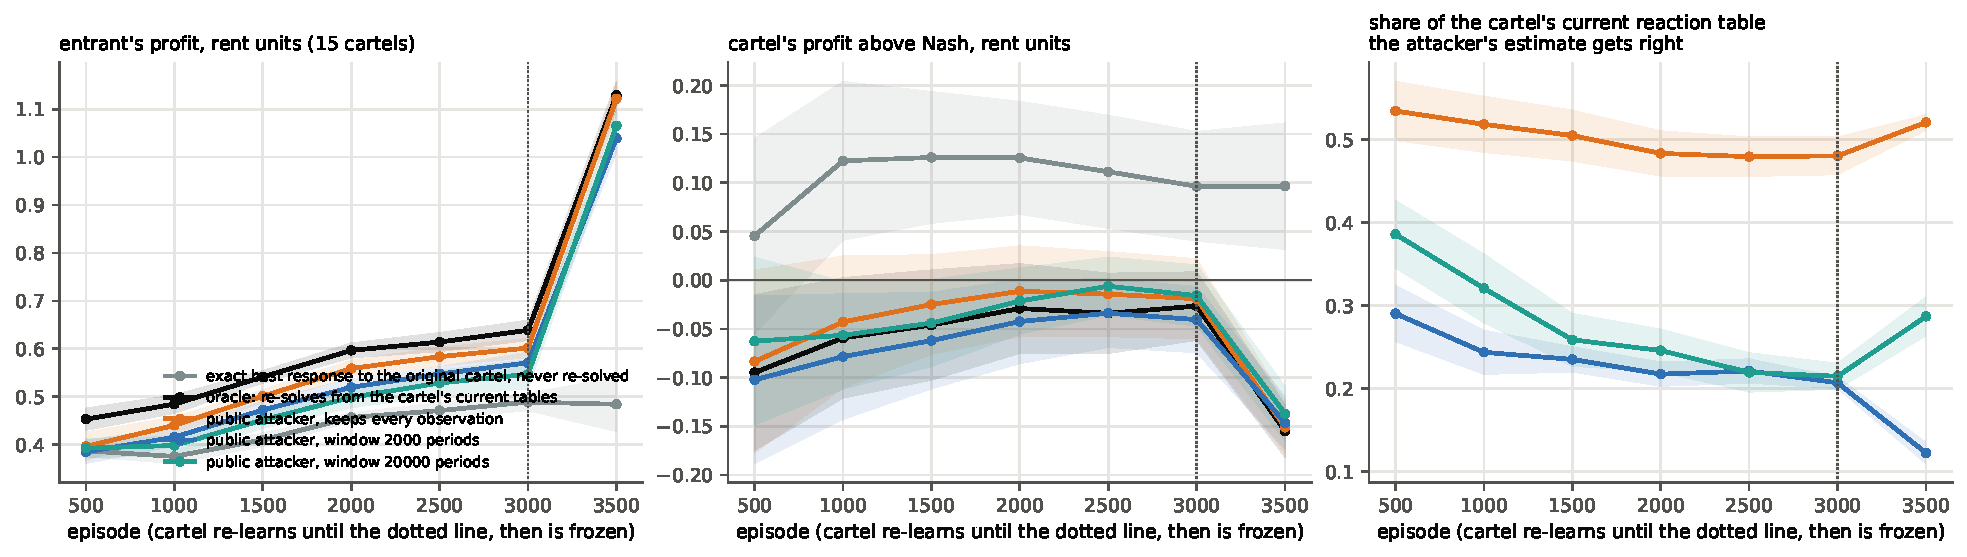
\includegraphics[width=0.9\textwidth]{fig_relearn_attack.pdf}
\takeaway{Learning lowers what the attacker can take (about 0.5 instead of 1.1), but the cartel earns about the Nash profit while it learns. We have run only the simplest version of the game.}
\note{A cartel that responds to the entrant's policy cannot be folded into P (Lecture 15 slide 9). Alternating the two sides for six rounds gave the same picture.}
\end{frame}

\begin{frame}{Identity as part of the state}
\partlabel{Data, Oct 6 -- Nov 1; RQ1}
\small
With public wallets, a maker's state can include each wallet's record, its fills and toxic fills: the lecture's belief $(n,h)$ for that wallet. On Hyperliquid, the makers who earn act on it.
\vspace{6pt}
\begin{columns}[T]
\begin{column}{0.32\textwidth}\stat{orange}{1.9--3.6$\times$}{fewer fills from previously toxic wallets for the top-10 makers}\end{column}
\begin{column}{0.32\textwidth}\stat{blue}{33 of 35}{coin-days on which the gap holds (four weeks)}\end{column}
\begin{column}{0.32\textwidth}\stat{aqua}{10 days}{for which a wallet's label stays useful}\end{column}
\end{columns}
\vspace{6pt}
\textbf{Open questions from the lecture.} Avoiding a wallet stops the feedback on it: is avoidance a trap (slide 37)? More information can lower the gains from trade in a game (slides 41--42): who bears it when wallets are public?
\takeaway{Public identity changes what the makers' state contains. Whether avoidance traps them is the next question.}
\note{Figure for questions: fig\_longwindow. Oct 29 stress episode: one identity-blind wallet absorbed the toxic flow.}
\end{frame}

\begin{frame}{The ordinary trader: who pays?}
\partlabel{The least-informed participant, same model}
\vspace{4pt}
\begin{columns}[T]
\begin{column}{0.58\textwidth}\centering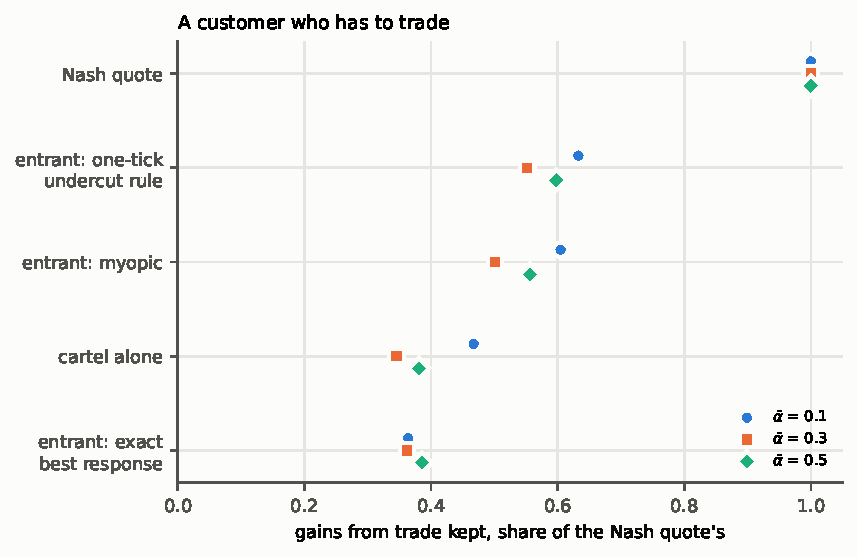
\includegraphics[width=\textwidth]{fig_retail_customer.pdf}\end{column}
\begin{column}{0.42\textwidth}\small
A customer who \textbf{has to trade} (moving savings in or out) is the model's uninformed taker. Her gains from trade fall as the quote widens.\\[5pt]
\stat{orange}{36--39\%}{of the Nash quote's gains left by the attack that is best for the attacker: no more than the cartel alone (35--47\%)}
\end{column}
\end{columns}
\takeaway{The attacker keeps the cartel wide and sits just inside it. The customer pays for both.}
\note{The myopic entrant, which pushes the cartel down, leaves her 50--60\%. 30 two-maker cartels, model paths.}
\end{frame}

\begin{frame}{Betting your savings without information: the ship again}
\partlabel{Lecture 15 part 2, with the trader as the ship}
\small
\begin{columns}[T]
\begin{column}{0.48\textwidth}
\begin{itemize}\setlength{\itemsep}{4pt}
\item A bet that is right with probability $p$ earns $(2p-1)\mu - x$: $\mu$ the mean price move, $x$ the half-spread.
\item Break-even: $p^* = \tfrac12 + x/(2\mu)$. One-tick book: $0.55$. Cartel's quotes: above 1.
\item She does not know $p$. Belief $(n,k)$: trades made, right calls. Trade = the strait (teaches), stop = the Cape (teaches nothing).
\end{itemize}
\end{column}
\begin{column}{0.52\textwidth}\centering
\footnotesize
\begin{tabular}{lccc}
\toprule
one year, optimistic prior & \multicolumn{2}{c}{no edge} & real edge \\
policy & profit & ruin & still trading \\
\midrule
never updates & $-25.0$ & 74\% & 100\% \\
myopic Bayesian & $-1.2$ & 0.3\% & 23\% \\
patient, $\delta=0.9$ & $-2.9$ & 1.0\% & 47\% \\
patient, $\delta=0.99$ & $-5.6$ & 3.8\% & 71\% \\
\bottomrule
\end{tabular}\\[3pt]
\raggedright profit in average price moves; savings 20 moves; real edge $p=0.6$.
\end{column}
\end{columns}
\takeaway{Without an edge, patience costs: information is only worth buying if an edge is plausible. With one, the myopic rule quits it 77\% of the time: the trap.}
\note{Stylised model, not investment advice. Rothschild (1974), as in the lecture.}
\end{frame}

\begin{frame}{Summary}
\partlabel{And what comes next}
\vspace{4pt}
\begin{columns}[T]
\begin{column}{0.25\textwidth}\rqbox{orange}{1~~Planning attacks}{The entrant solves an MDP. Looking ahead adds 0.13--0.30.}\end{column}
\begin{column}{0.25\textwidth}\rqbox{blue}{2~~The model is public}{The cartel's reaction is on the public book.}\end{column}
\begin{column}{0.25\textwidth}\rqbox{aqua}{3~~Learners are players}{A game. Learning did not bring the rent back.}\end{column}
\begin{column}{0.25\textwidth}\rqbox{navy}{4~~The customer pays}{The best attack leaves her no better off. Updating protects savings.}\end{column}
\end{columns}
\vspace{8pt}
\small\textbf{Next:} full-size runs; the trap question on order-level data; preprint in mid-December.\\[3pt]
\centering\texttt{github.com/pradeepu191/wargame}
\note{Close.}
\end{frame}

\begin{frame}{Backup: also explored, not claimed here}
\partlabel{Preliminary; in the repository}
\small
\begin{itemize}\setlength{\itemsep}{5pt}
\item \textbf{One-tick books (queue game).} When the spread cannot move, makers only choose to keep an order standing or not. Steering the incumbents gained nothing (3 seeds).
\item \textbf{Request allowance.} A cap on order placements removed the identity selector's edge (3 seeds).
\item \textbf{Defences on one frontier.} Maker and exchange rules against the strongest attackers; run in progress.
\end{itemize}
\vspace{4pt}
Details: \texttt{results/REPLICATION\_NOTES.md}, sections dated Nov 15--16.
\note{Only if asked.}
\end{frame}
\end{document}"
\usetheme[progressbar=frametitle,numbering=fraction,block=fill,sectionpage=none]{metropolis}
\usepackage[T1]{fontenc}
\usepackage{helvet}\renewcommand{\familydefault}{\sfdefault}
\usepackage{amsmath,amssymb}
\usepackage{booktabs}
\usepackage{tikz}
\usetikzlibrary{arrows.meta,positioning,calc,fit}
\tikzset{pl/.style={draw=#1,fill=#1!12,rounded corners=3pt,text width=3.5cm,align=left,inner sep=7pt}}
\usepackage{graphicx}
\usepackage[skins]{tcolorbox}
\ifdefined\shownotes
  \usepackage{pgfpages}
  \setbeameroption{show notes on second screen=right}
  \setbeamertemplate{note page}[plain]
  \setbeamerfont{note page}{size=\small}
\fi
\graphicspath{{../results/}{../results/live_2026_10/}}
\definecolor{ink}{HTML}{0b0b0b}
\definecolor{muted}{HTML}{52514e}
\definecolor{navy}{HTML}{0d366b}
\definecolor{blue}{HTML}{2a78d6}
\definecolor{paleblue}{HTML}{eaf2fc}
\definecolor{orange}{HTML}{eb6834}
\definecolor{paleorange}{HTML}{fdf0e9}
\definecolor{aqua}{HTML}{1baf7a}
\definecolor{red}{HTML}{e34948}
\definecolor{grey}{HTML}{9a9890}
\definecolor{paper}{HTML}{fcfcfb}
\setbeamercolor{normal text}{fg=ink,bg=paper}
\setbeamercolor{frametitle}{bg=navy,fg=white}
\setbeamercolor{progress bar}{fg=orange,bg=navy!25}
\setbeamercolor{alerted text}{fg=orange}
\setbeamercolor{block title}{bg=paleblue,fg=navy}
\setbeamercolor{block body}{bg=paleblue,fg=ink}
\setbeamercolor{itemize item}{fg=blue}
\setbeamercolor{enumerate item}{fg=blue}
\setbeamercolor{title separator}{fg=orange}
\setbeamerfont{frametitle}{size=\large,series=\bfseries}
\setbeamerfont{caption}{size=\scriptsize}
\setbeamertemplate{caption}{\insertcaption}
\setbeamertemplate{itemize items}{\textcolor{blue}{$\blacktriangleright$}}
\setlength{\leftmargini}{1.1em}
\newcommand{\Fanon}{\mathcal{F}^{\mathrm{anon}}}
\newcommand{\Fid}{\mathcal{F}^{\mathrm{id}}}
\newcommand{\For}{\mathcal{F}^{\mathrm{oracle}}}
\newcommand{\LBR}{L_{\mathrm{BR}}}
\newcommand{\takeaway}[1]{\vspace{3pt}\begin{tcolorbox}[enhanced,colback=paleorange,colframe=paleorange,borderline west={2.5pt}{0pt}{orange},boxrule=0pt,arc=1.5pt,left=6pt,right=6pt,top=3pt,bottom=3pt]\small\textbf{#1}\end{tcolorbox}}
\newcommand{\rqbox}[3]{\begin{tcolorbox}[enhanced,colback=paleblue,colframe=paleblue,borderline north={2.5pt}{0pt}{#1},boxrule=0pt,arc=1.5pt,left=6pt,right=6pt,top=5pt,bottom=5pt,height=2.6cm,valign=top]\raggedright\textcolor{#1}{\textbf{#2}}\par\vspace{3pt}\small #3\end{tcolorbox}}
\newcommand{\stat}[3]{\begin{tcolorbox}[enhanced,colback=paleblue,colframe=paleblue,borderline north={2.5pt}{0pt}{#1},boxrule=0pt,arc=1.5pt,left=5pt,right=5pt,top=4pt,bottom=4pt]\centering{\LARGE\textbf{\textcolor{#1}{#2}}}\par\vspace{2pt}{\footnotesize #3}\end{tcolorbox}}
\newcommand{\partlabel}[1]{\vspace{-10pt}\par\noindent\hfill{\scriptsize\textcolor{muted}{\textsc{#1}}}\par\vspace{-4pt}}
\newcommand{\subline}[1]{\par\vspace{3pt}{\small #1}\par}

\title{\huge Can an attacker plan against learning market makers?}
\subtitle{The entrant's problem as a Markov decision problem\\ {\small\textcolor{white!70!navy}{Rent or toxicity: strategic exploitability of learning market makers with public wallet information}}}
\author{Deepu Pradeep \quad Miguel Betran Menz}
\institute{6.S974 Games, Learning, and Security, Workshop 2 (draft)\\ Example 4: an algorithmic market with adaptive agents}
\date{November 2026}

\begin{document}
{\setbeamercolor{background canvas}{bg=navy}\setbeamercolor{normal text}{fg=white}\setbeamercolor{title}{fg=white}\setbeamercolor{subtitle}{fg=white!85!navy}\setbeamercolor{author}{fg=white}\setbeamercolor{institute}{fg=white!80!navy}\setbeamercolor{date}{fg=white!80!navy}\usebeamercolor[fg]{normal text}
\maketitle}

\begin{frame}{The words we use today}
\partlabel{Recap from Workshop 1}
\small
\begin{columns}[T]
\begin{column}{0.5\textwidth}
\begin{itemize}\setlength{\itemsep}{4pt}
\item \textbf{Maker}: posts standing offers to buy and sell. \textbf{Taker}: accepts one.
\item \textbf{Half-spread} $h$: how far a maker's prices sit from the mid, in \textbf{ticks} (smallest price step).
\item \textbf{Nash quote} $h^C$: break-even. \textbf{Monopoly quote} $h^M$: what a single maker would choose.
\end{itemize}
\end{column}
\begin{column}{0.5\textwidth}
\begin{itemize}\setlength{\itemsep}{4pt}
\item \textbf{Cartel}: learning makers that settle above Nash without communicating. \textbf{Rent}: their profit above Nash.
\item \textbf{Entrant}: the attacker, one more maker.
\item \textbf{Rent units}: profit divided by (monopoly $-$ Nash) profit. 1 is the whole rent.
\end{itemize}
\end{column}
\end{columns}
\takeaway{Workshop 1: the rent exists, and an entrant that knows how the cartel reacts takes all of it.}
\note{One slide to recall the vocabulary. The planning words come from Lecture 15 and are defined as we go.}
\end{frame}

\begin{frame}{The entrant's quote changes the cartel it faces tomorrow}
\partlabel{The frame of Lecture 15}
\centering
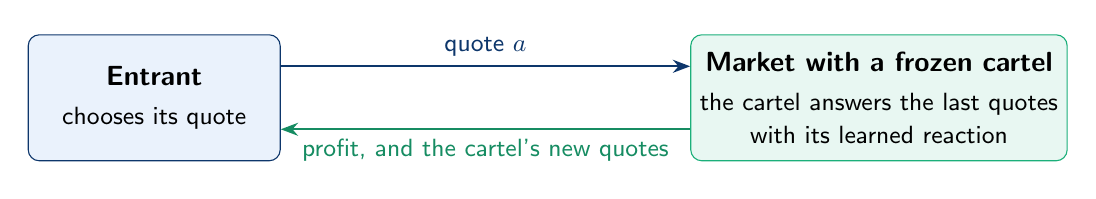
\begin{tikzpicture}[node distance=5.2cm, >={Stealth[length=2.2mm]}]
\node[draw=navy,fill=paleblue,rounded corners=4pt,minimum width=3.2cm,minimum height=1.6cm,align=center] (E) {\textbf{Entrant}\\[2pt]\small chooses its quote};
\node[draw=aqua,fill=aqua!10,rounded corners=4pt,minimum width=4.2cm,minimum height=1.6cm,align=center,right=of E] (M) {\textbf{Market with a frozen cartel}\\[2pt]\small the cartel answers the last quotes\\ \small with its learned reaction};
\draw[->,navy,thick] ([yshift=4mm]E.east) -- node[above]{\small quote $a$} ([yshift=4mm]M.west);
\draw[->,aqua!80!black,thick] ([yshift=-4mm]M.west) -- node[below]{\small profit, and the cartel's new quotes} ([yshift=-4mm]E.east);
\end{tikzpicture}
\vspace{6pt}
\begin{itemize}\small\setlength{\itemsep}{3pt}
\item Should the entrant always take the quote that earns most today?
\item What does it need to know, and can it learn that from public information?
\item What changes when the cartel keeps learning?
\item And for the least-informed participant: what is optimal, and who pays?
\end{itemize}
\takeaway{Three questions about the attacker, one per part of the lecture, and one about the ordinary trader.}
\note{Same picture as slide 2 of Lecture 15, with the ship replaced by the entrant and the insurance quote by the cartel's quote.}
\end{frame}

\begin{frame}{Against a frozen cartel, the entrant faces an MDP}
\partlabel{Lecture 15: finite MDP; the opponent as part of P}
\small
\begin{columns}[T]
\begin{column}{0.56\textwidth}
\begin{itemize}\setlength{\itemsep}{4pt}
\item \textbf{State} $x$: last period's quotes $(h_1,h_2,h_e)$, $24^3$ states.
\item \textbf{Action} $a$: the entrant's half-spread, $1,\dots,24$.
\item \textbf{Transitions} $P$: the cartel answers $x$ with its reaction $g(x)$; next state $(g(x),a)$. Deterministic.
\item \textbf{Reward} $r(x,a)$: expected profit this period, closed form.
\item \textbf{Turn limit}: 100 periods per episode.
\end{itemize}
\end{column}
\begin{column}{0.44\textwidth}
\textbf{Why this state is valid.} Each learner chooses from its own last quote and the best rival quote. Last period's quotes predict the cartel's answer and the profit.\\[6pt]
\textbf{Why the cartel is part of $P$.} Frozen, it does not respond to the entrant's \emph{policy}, only to its last quote, like the missiles of the lecture's example.
\end{column}
\end{columns}
\takeaway{The exact best response of Workshop 1 is backward induction on this MDP: value iteration with k = periods left.}
\note{Lecture 15 slides 7, 9, 12. The state must make the rest of the history irrelevant; here it does, because the learners' own state is the last quotes.}
\end{frame}

\begin{frame}{A quote that earns more today gives a policy that earns less}
\partlabel{Lecture 15 slide 15, on one of our cartels}
\small
\begin{columns}[T]
\begin{column}{0.5\textwidth}\centering
\textbf{Myopic: best profit today}\\[3pt]
\begin{tabular}{cccc}
\toprule
period & cartel & entrant & profit \\
\midrule
0 & 15, 17 & 13 & 1.21 \\
1 & 16, 13 & 12 & 1.21 \\
2 & 18, \textcolor{red}{9} & 8 & \textcolor{red}{1.05} \\
3 & \textcolor{red}{7}, 11 & 6 & \textcolor{red}{0.86} \\
\bottomrule
\end{tabular}
\end{column}
\begin{column}{0.5\textwidth}\centering
\textbf{Optimal: best total}\\[3pt]
\begin{tabular}{cccc}
\toprule
period & cartel & entrant & profit \\
\midrule
0 & 15, 17 & 12 & 1.21 \\
1 & 21, 23 & 14 & \textcolor{orange}{1.20} \\
2 & 24, 14 & 12 & 1.21 \\
3 & 14, 22 & 13 & 1.21 \\
\bottomrule
\end{tabular}
\end{column}
\end{columns}
\vspace{6pt}
Quotes in ticks; profit in rent units. In period 1 the optimal entrant gives up $0.01$ today, and the cartel stays wide.
\takeaway{The myopic entrant pushes the cartel down to 7--9 ticks. The optimal one keeps it wide and stays just inside it.}
\note{Cartel cfl\_exp2 alpha 0.1 seed 0, from python experiments/planning\_view.py. Read it like the value-iteration table of the lecture.}
\end{frame}

\begin{frame}{How much is looking ahead worth?}
\partlabel{30 two-maker cartels, ten per toxicity level}
\centering\small
\begin{tabular}{lcccc}
\toprule
policy & $\bar\alpha=0.1$ & $0.3$ & $0.5$ & simulator \\
\midrule
one-tick undercut (no model) & 0.53 & 0.48 & 0.46 & 0.50 \\
myopic (knows $P$, $\delta=0$) & 0.91 & 0.94 & 0.95 & 0.94 \\
$\delta=0.5$ & 1.20 & 1.08 & 1.16 & 1.15 \\
$\delta=0.9$ & 1.21 & 1.08 & 1.17 & 1.15 \\
optimal (100-period total) & 1.21 & 1.08 & 1.17 & 1.15 \\
\bottomrule
\end{tabular}\\[4pt]
\raggedright\footnotesize Entrant's profit per period, rent units. Columns 2--4: on the model from the starting state. Simulator: the same policies in the real simulator, toxicity levels pooled.
\takeaway{Knowing the cartel doubles the take. Looking ahead adds the rest, and a discount of 0.5 is already enough.}
\note{Lecture 15 slides 34--36: patience moves the decision. Here most of the gain comes with the first step of looking ahead.}
\end{frame}

\begin{frame}{Live: the model, period by period}
\partlabel{Demonstration}
\begin{columns}[T]
\begin{column}{0.55\textwidth}\small
\texttt{demo/index.html} replays recorded runs of the real simulator.
\begin{itemize}\setlength{\itemsep}{3pt}
\item makers' quotes against the Nash and monopoly quotes
\item each taker's order, coloured after the fact
\item running profit per maker
\end{itemize}
Controls: play, step, seek, \textbf{playback rate} 1--200 periods per second, two runs side by side.
\end{column}
\begin{column}{0.45\textwidth}\small
\textbf{Show, in this order}
\begin{enumerate}\setlength{\itemsep}{3pt}
\item The cartel alone (5 periods/s)
\item Myopic and optimal entrant side by side (step through 10 periods)
\item The public attacker: probing, then planning
\item Betting savings: never updates beside the myopic Bayesian; then a real edge, myopic beside patient (the trap)
\end{enumerate}
\end{column}
\end{columns}
\takeaway{The replay holds no model logic: a test pins it to the experiment code.}
\note{Switch to the browser. Backup if there is no browser: the GIFs in results/demo.}
\end{frame}

\begin{frame}{Without the model: build it from the public book}
\partlabel{Model-based with a learned model; 60 cartels}
\vspace{6pt}
\begin{columns}[T]
\begin{column}{0.58\textwidth}\centering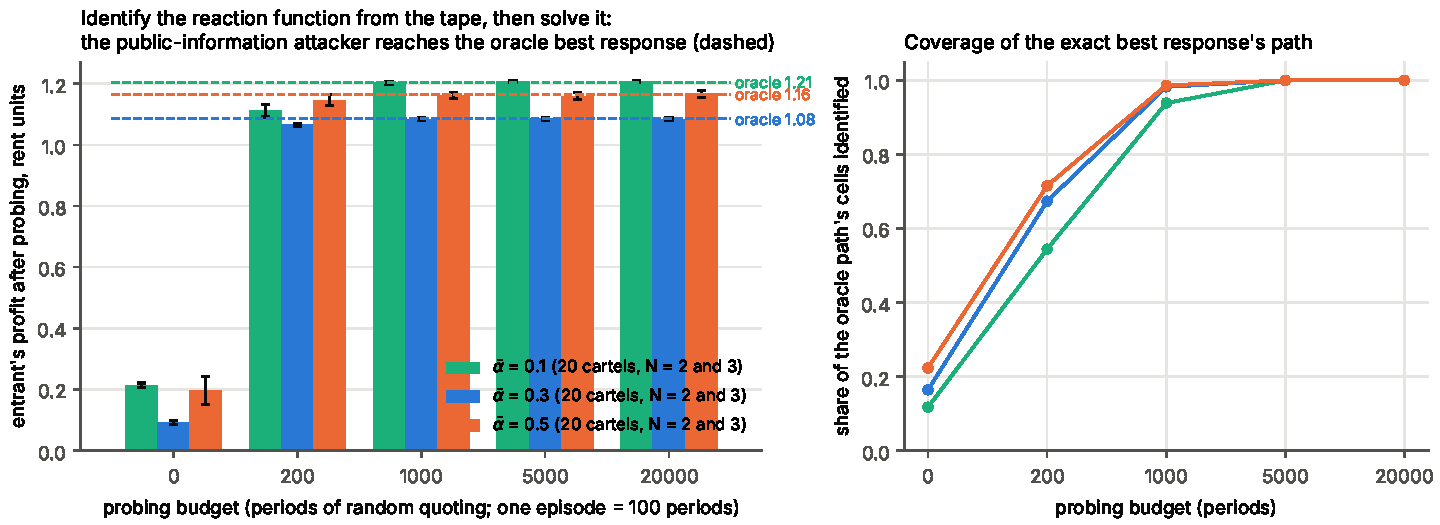
\includegraphics[width=\textwidth]{fig_public_attacker.pdf}\end{column}
\begin{column}{0.42\textwidth}\small
Every value of $P$ is on the public book: the cartel's answer appears next to the quotes it answered.\\[4pt]
Quote at random for a \textbf{probing budget}, record the answers, plan on the estimate.\\[4pt]
\stat{orange}{1000 periods}{of probing match planning with the true $P$}
\end{column}
\end{columns}
\takeaway{Probing costs profit, so the best budget is two to ten episodes. Feedback is selective: only visited states are learned.}
\note{Lecture 15: model-based planning. Next lecture is model-free; the cartel's own learners are model-free Q-learners.}
\end{frame}

\begin{frame}{When the cartel keeps learning, it is a player}
\partlabel{The game; 15 two-maker cartels, laptop size}
\centering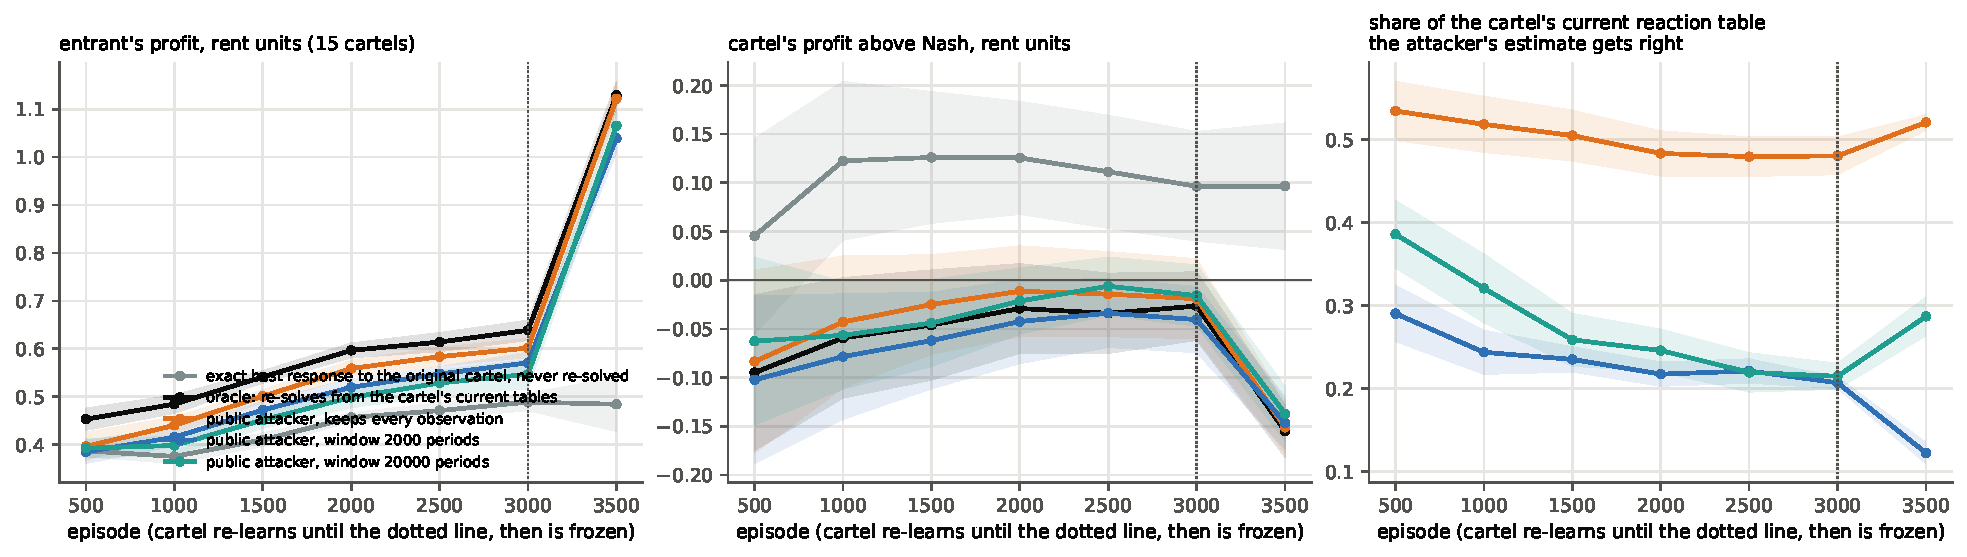
\includegraphics[width=0.9\textwidth]{fig_relearn_attack.pdf}
\takeaway{Learning lowers what the attacker can take (about 0.5 instead of 1.1), but the cartel earns about the Nash profit while it learns. We have run only the simplest version of the game.}
\note{A cartel that responds to the entrant's policy cannot be folded into P (Lecture 15 slide 9). Alternating the two sides for six rounds gave the same picture.}
\end{frame}

\begin{frame}{Identity as part of the state}
\partlabel{Data, Oct 6 -- Nov 1; RQ1}
\small
With public wallets, a maker's state can include each wallet's record, its fills and toxic fills: the lecture's belief $(n,h)$ for that wallet. On Hyperliquid, the makers who earn act on it.
\vspace{6pt}
\begin{columns}[T]
\begin{column}{0.32\textwidth}\stat{orange}{1.9--3.6$\times$}{fewer fills from previously toxic wallets for the top-10 makers}\end{column}
\begin{column}{0.32\textwidth}\stat{blue}{33 of 35}{coin-days on which the gap holds (four weeks)}\end{column}
\begin{column}{0.32\textwidth}\stat{aqua}{10 days}{for which a wallet's label stays useful}\end{column}
\end{columns}
\vspace{6pt}
\textbf{Open questions from the lecture.} Avoiding a wallet stops the feedback on it: is avoidance a trap (slide 37)? More information can lower the gains from trade in a game (slides 41--42): who bears it when wallets are public?
\takeaway{Public identity changes what the makers' state contains. Whether avoidance traps them is the next question.}
\note{Figure for questions: fig\_longwindow. Oct 29 stress episode: one identity-blind wallet absorbed the toxic flow.}
\end{frame}

\begin{frame}{The ordinary trader: who pays?}
\partlabel{The least-informed participant, same model}
\vspace{4pt}
\begin{columns}[T]
\begin{column}{0.58\textwidth}\centering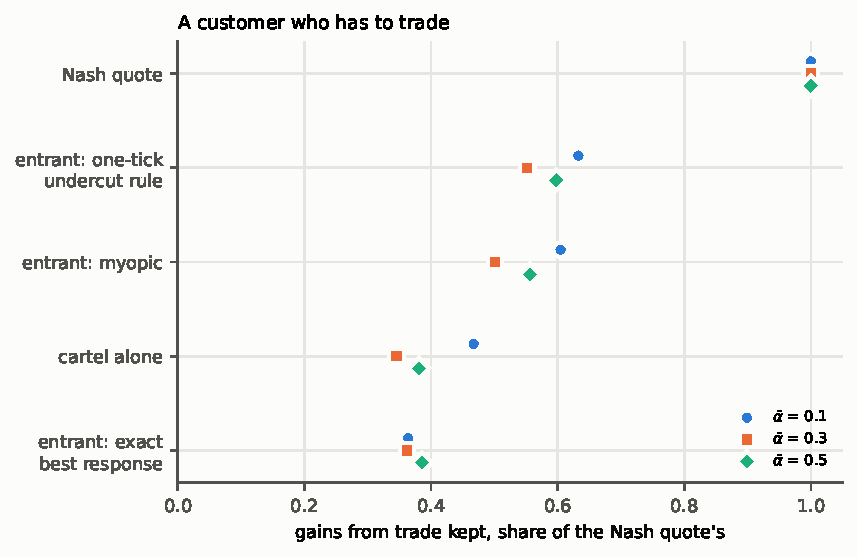
\includegraphics[width=\textwidth]{fig_retail_customer.pdf}\end{column}
\begin{column}{0.42\textwidth}\small
A customer who \textbf{has to trade} (moving savings in or out) is the model's uninformed taker. Her gains from trade fall as the quote widens.\\[5pt]
\stat{orange}{36--39\%}{of the Nash quote's gains left by the attack that is best for the attacker: no more than the cartel alone (35--47\%)}
\end{column}
\end{columns}
\takeaway{The attacker keeps the cartel wide and sits just inside it. The customer pays for both.}
\note{The myopic entrant, which pushes the cartel down, leaves her 50--60\%. 30 two-maker cartels, model paths.}
\end{frame}

\begin{frame}{Betting your savings without information: the ship again}
\partlabel{Lecture 15 part 2, with the trader as the ship}
\small
\begin{columns}[T]
\begin{column}{0.48\textwidth}
\begin{itemize}\setlength{\itemsep}{4pt}
\item A bet that is right with probability $p$ earns $(2p-1)\mu - x$: $\mu$ the mean price move, $x$ the half-spread.
\item Break-even: $p^* = \tfrac12 + x/(2\mu)$. One-tick book: $0.55$. Cartel's quotes: above 1.
\item She does not know $p$. Belief $(n,k)$: trades made, right calls. Trade = the strait (teaches), stop = the Cape (teaches nothing).
\end{itemize}
\end{column}
\begin{column}{0.52\textwidth}\centering
\footnotesize
\begin{tabular}{lccc}
\toprule
one year, optimistic prior & \multicolumn{2}{c}{no edge} & real edge \\
policy & profit & ruin & still trading \\
\midrule
never updates & $-25.0$ & 74\% & 100\% \\
myopic Bayesian & $-1.2$ & 0.3\% & 23\% \\
patient, $\delta=0.9$ & $-2.9$ & 1.0\% & 47\% \\
patient, $\delta=0.99$ & $-5.6$ & 3.8\% & 71\% \\
\bottomrule
\end{tabular}\\[3pt]
\raggedright profit in average price moves; savings 20 moves; real edge $p=0.6$.
\end{column}
\end{columns}
\takeaway{Without an edge, patience costs: information is only worth buying if an edge is plausible. With one, the myopic rule quits it 77\% of the time: the trap.}
\note{Stylised model, not investment advice. Rothschild (1974), as in the lecture.}
\end{frame}

\begin{frame}{Summary}
\partlabel{And what comes next}
\vspace{4pt}
\begin{columns}[T]
\begin{column}{0.25\textwidth}\rqbox{orange}{1~~Planning attacks}{The entrant solves an MDP. Looking ahead adds 0.13--0.30.}\end{column}
\begin{column}{0.25\textwidth}\rqbox{blue}{2~~The model is public}{The cartel's reaction is on the public book.}\end{column}
\begin{column}{0.25\textwidth}\rqbox{aqua}{3~~Learners are players}{A game. Learning did not bring the rent back.}\end{column}
\begin{column}{0.25\textwidth}\rqbox{navy}{4~~The customer pays}{The best attack leaves her no better off. Updating protects savings.}\end{column}
\end{columns}
\vspace{8pt}
\small\textbf{Next:} full-size runs; the trap question on order-level data; preprint in mid-December.\\[3pt]
\centering\texttt{github.com/pradeepu191/wargame}
\note{Close.}
\end{frame}

\begin{frame}{Backup: also explored, not claimed here}
\partlabel{Preliminary; in the repository}
\small
\begin{itemize}\setlength{\itemsep}{5pt}
\item \textbf{One-tick books (queue game).} When the spread cannot move, makers only choose to keep an order standing or not. Steering the incumbents gained nothing (3 seeds).
\item \textbf{Request allowance.} A cap on order placements removed the identity selector's edge (3 seeds).
\item \textbf{Defences on one frontier.} Maker and exchange rules against the strongest attackers; run in progress.
\end{itemize}
\vspace{4pt}
Details: \texttt{results/REPLICATION\_NOTES.md}, sections dated Nov 15--16.
\note{Only if asked.}
\end{frame}
\end{document}